Cluster algebras, introduced by Fomin and Zelevinsky~\cite{FZ1_2002}, are
commutative algebras with specific generators, called \emph{cluster
	variables}, defined recursively.
In this section, we recall basic notions in the theory of cluster algebras.
For more details, we refer the reader to~\cite{FZ1_2002, FZ2_2003, FZ4_2007}.

Throughout this section, we fix $m, n \in \Z_{>0}$ such that $n \leq m$, and
we let $\field$ be the rational function field with $m$ independent
variables over $\bbC$.


\subsection{Basics on cluster algebras}


\begin{definition}[{cf. \cite{FZ1_2002, FZ2_2003, FZ4_2007}}]\label{definition:seeds}
A seed and $Y$-seed are defined as follows.
\begin{enumerate}
\item	A \emph{seed} $(\bfx, \qbasis)$ is a pair of 
	\begin{itemize}
		\item a tuple $\bfx = (x_1,\dots,x_m)$ of algebraically
		independent generators of $\field$, that is, 
		$\field = \bbC(x_1,\dots,x_m)$;
		\item an $m \times n$ integer matrix $\qbasis = (b_{i,j})_{i,j}$ such
		that the \emph{principal part} $\qbasispr \colonequals
		(b_{i,j})_{1\leq i,j\leq n}$ is skew-symmetrizable, that is, there
		exist positive integers $d_1,\dots,d_n$ such that
\[		
\textrm{diag}(d_1,\dots,d_n) \cdot \qbasispr 
\]
		is a
		skew-symmetric matrix.
	\end{itemize}
	We refer to $\bfx$ as the \emph{cluster} of a seed $(\bfx, \qbasis)$, to elements $x_1,\dots,x_m$ as \emph{cluster variables}, and to
	$\qbasis$ as the \emph{exchange matrix}. Moreover, we call $x_1,\dots,x_n$
	\emph{unfrozen} (or, \emph{mutable}) variables and $x_{n+1},\dots,x_m$
	\emph{frozen} variables.
\item A \emph{$Y$-seed} $(\bfy,\qbasispr)$ is a pair of an $n$-tuple $\bfy=(y_1,\dots,y_n)$ of elements in $\field$ and an $n\times n$ skew-symmetrizable matrix $\qbasispr$. 
We call $\bfy$ the \emph{coefficient tuple} of a $Y$-seed $(\bfy, \qbasispr)$ and call $y_1,\dots,y_n$ \emph{coefficients}.
\end{enumerate}
\end{definition}
We say that two seeds $(\bfx, \qbasis)$ and $(\bfx', \qbasis')$ are \textit{equivalent}, denoted by $(\bfx, \qbasis)\sim(\bfx', \qbasis')$ if there exists a permutation $\sigma$ on $[m]$ such that $\sigma|_{[n]}=[n]$, 
\[
x_i' = x_{\sigma(i)}\quad \text{ and } \quad b_{i,j}' = b_{\sigma(i),\sigma(j)} \quad \text{ for }1\le i\le m, 1\le j\le n,
\]
where $\bfx = (x_{1},\dots,x_{m})$, $\bfx' = (x_1',\dots,x_m')$, $\qbasis = (b_{i,j})$, and $\qbasis' = (b_{i,j}')$. Similarly,
two $Y$-seeds $(\bfy,\qbasispr)$ and $(\bfy',\qbasispr')$ are \emph{equivalent} and denoted by $(\bfy,\qbasispr)\sim(\bfy',\qbasispr')$ if there exists a permutation $\sigma$ on $[n]$ such that %$\sigma|_{[n]}=[n]$,
\[
y_i' = y_{\sigma(i)}\quad\text{and}\quad
b_{i,j}' = b_{\sigma(i),\sigma(j)}\quad\text{for }1\le i,j \le n.
\]

To define cluster algebras, we introduce mutations on exchange matrices, and quivers, and seeds as follows. 
\begin{enumerate}
\item (Mutation on exchange matrices)
For an exchange matrix $\qbasis$ and $1 \le k \le n$, the mutation $\mu_k(\qbasis) = (b_{i,j}')$ is defined as follows.
\[
b_{i,j}' = \begin{cases}
-b_{i,j} & \text{ if } i = k \text{ or } j = k, \\
\displaystyle b_{i,j} + \frac{|b_{i,k}| b_{k,j} + b_{i,k} | b_{k,j}|} {2} & \text{ otherwise}.
\end{cases}
\]
We say that \emph{$\qbasis' =(b_{i,j}')$ is the mutation of $\qbasis$ at $k$}.
\item (Mutation on quivers)
We call a finite directed multigraph $\quiver$ a \emph{quiver} if it does not have
oriented cycles of length at most $2$. The adjacency matrix $\qbasis(\quiver)$ of a
quiver is always skew-symmetric. Moreover, $\mu_k(\qbasis(\quiver))$ is again 
the adjacency matrix of a quiver $\quiver'$. We define $\mu_k(\quiver)$ to be 
the quiver satisfying 
\[
 \qbasis(\mu_k(\quiver)) = \mu_k(\qbasis(\quiver)),
\]
and say that \emph{$\mu_k(\quiver)$ is the mutation of $\quiver$ at $k$}.
\item (Mutation on seeds)	For a seed $(\bfx, \qbasis)$ and an integer $1 \leq k \leq n$, the \emph{mutation} $\mutation_k(\bfx, \qbasis) = (\bfx', \mu_k(\qbasis))$ is defined as follows: 
\begin{equation*}%\label{eq_mutation_on_seed_A}
x_i' = \begin{cases}
x_i &\text{ if } i \neq k,\\
\displaystyle 
x_k^{-1}\left( \prod_{b_{j,k} > 0} x_j^{b_{j,k}} + \prod_{b_{j,k} < 0}x_j^{-b_{j,k}}
\right) & \text{ otherwise}.
\end{cases}
\end{equation*}
\item (Mutation on $Y$-seeds)
The \emph{$Y$-seed mutation} (or, \emph{cluster $\mathcal{X}$-mutation}, \emph{$\mathcal{X}$-cluster mutation}) on a $Y$-seed $(\bfy, \qbasispr)$ at $k\in[n]$ is a $Y$-seed $(\bfy'=(y_1',\dots, y_n'),\qbasispr'=\mu_k(\qbasispr))$, where for each $1 \le i\le n$,
\[
y_i' = \begin{cases}
    \displaystyle {y}_{i} {y}_{k}^{\max\{b_{i,k},0\}}(1+{y}_{k})^{-b_{i,k}} & \text{ if }i \neq k, \\
   {y}_{k}^{-1} &\text{ otherwise}.
\end{cases}
\]


\end{enumerate}


\begin{example}\label{example_mutation_skewsymmetrizable}
Let $n = m = 2$. Suppose that an initial seed is given by
\[
(\bfx_{t_0}, \qbasis_{t_0}) = \left(
(x_1,x_2), \begin{pmatrix}
0 & 1 \\ -3 & 0
\end{pmatrix}
\right).
\]
Considering mutations $\mu_1(\bfx_{t_0}, \qbasis_{t_0})$ and $\mu_2\mu_1(\bfx_{t_0}, \qbasis_{t_0})$, we obtain the following.
\begin{align*}
\mu_1(\bfx_{t_0}, \qbasis_{t_0}) &= \left(
\left(
\frac{1+x_2^3}{x_1},x_2
\right), \begin{pmatrix}
0 & -1 \\3 & 0
\end{pmatrix}
\right),\\
\mu_2\mu_1(\bfx_{t_0}, \qbasis_{t_0}) &= \left(
\left(
\frac{1+x_2^3}{x_1}, \frac{1+x_1+x_2^3}{x_1x_2}
\right),
\begin{pmatrix}
0 & 1  \\ -3 & 0
\end{pmatrix}
\right).
\end{align*}
\end{example}


\begin{remark}\label{rmk_mutation_on_quivers}
Let $k$ be a vertex in a quiver $\quiver$ on $[m]$.
The mutation $\mutation_k(\quiver)$ can also be described via a sequence of three steps:
\begin{enumerate}
\item For each directed two-arrow path $i \to k \to j$, add a new arrow $i \to j$.
\item Reverse the direction of all arrows incident to the vertex $k$.
\item Repeatedly remove directed $2$-cycles until unable to do so.
\end{enumerate}
\end{remark}
\begin{remark}\label{rmk_mutation_commutes}
Let $\qbasis = (b_{i,j})$ be an exchange matrix of size $m \times n$.
For $k,\ell \in [n]$, if $b_{k,\ell} = b_{\ell,k} = 0$, then the mutations at $k$ and $\ell$ commute with each other: $\mutation_{\ell}(\mutation_k(\qbasis)) = \mutation_k(\mutation_{\ell}(\qbasis))$. 
Similarly, for a quiver $\quiver$ on $[m]$, if there does not exist an arrow connecting mutable vertices $k$ and $\ell$, then we have $\mutation_{\ell}(\mutation_k(\quiver)) = \mutation_k(\mutation_{\ell}(\quiver))$.
\end{remark}

We say a quiver $\quiver'$ is \emph{mutation equivalent} to another quiver $\quiver$ if 
there exists a sequence  of mutations $\mutation_{j_1},\dots,\mutation_{j_{\ell}}$ 
which connects $\quiver'$ and $\quiver$, that is,
\[
\quiver' = (\mutation_{j_{\ell}} \cdots \mutation_{j_1})(\quiver).
\]
Similarly, we say an exchange matrix $\qbasis'$ is \emph{mutation equivalent} to another matrix $\qbasis$ if $\qbasis'$ is obtained by applying a sequence of mutations to $\qbasis$. 


An immediate check shows that $\mutation_k(\bfx,\qbasis)$ is again a seed $\mutation_k(\bfy,\qbasispr)$ is a $Y$-seed, and a mutation is an involution, that is, its square is the identity.
Also, note that the mutation on seeds does not change frozen variables $x_{n+1},\dots,x_m$.
Let $\mathbb{T}_n$ denote the $n$-regular tree whose edges are labeled by $1,\dots,n$. Except for $n = 1$, there are infinitely many vertices on the tree $\mathbb{T}_n$. For example, we present regular trees $\mathbb{T}_2$ and $\mathbb{T}_3$ in Figure~\ref{figure_regular_trees_2_and_3}.
\begin{figure}
	\begin{tabular}{cc}
		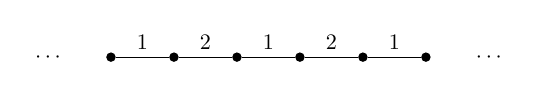
\begin{tikzpicture}
		\tikzset{every node/.style={scale=0.8}}
		\tikzset{cnode/.style = {circle, fill,inner sep=0pt, minimum size= 1.5mm}}
		\node[cnode] (1) {};
		\node[cnode, right of=1 ] (2) {};
		\node[cnode, right of=2 ] (3) {};
		\node[cnode, right of=3 ] (4) {};	
		\node[cnode, right of=4 ] (5) {};	
		\node[cnode, right of=5 ] (6) {};	
		
		\node[left of=1] {$\cdots$};
		\node[right of=6] {$\cdots$};
		
		\draw (1)--(2) node[above, midway] {$1$};
		\draw (2)--(3) node[above, midway] {$2$};
		\draw (3)--(4) node[above, midway] {$1$};
		\draw (4)--(5) node[above, midway] {$2$};
		\draw (5)--(6) node[above, midway] {$1$};
		\end{tikzpicture} &
		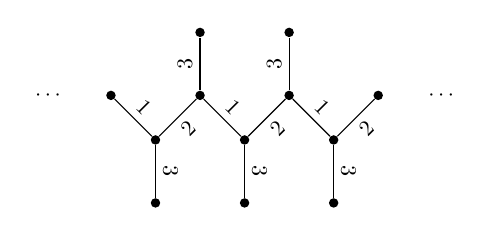
\begin{tikzpicture}
			\tikzset{every node/.style={scale=0.8}}
		\tikzset{cnode/.style = {circle, fill,inner sep=0pt, minimum size= 1.5mm}}
		\node[cnode] (1) {};
		\node[cnode, below right of =1] (2) {};
		\node[cnode, below of =2] (3) {};
		\node[cnode, above right of=2] (4){};
		\node[cnode, above of =4] (5) {};
		\node[cnode, below right of = 4] (6) {};
		\node[cnode, below of= 6] (7) {};
		\node[cnode, above right of = 6] (8) {};
		\node[cnode, above of = 8] (9) {};
		\node[cnode, below right of = 8] (10) {};
		\node[cnode, below of = 10] (11) {};
		\node[cnode, above right of = 10] (12) {};
		
		\node[left of = 1] {$\cdots$};
		\node[right of = 12] {$\cdots$};
		
		\draw (1)--(2) node[above, midway, sloped] {$1$};
		\draw (4)--(6) node[above, midway, sloped] {$1$};
		\draw (8)--(10) node[above, midway, sloped] {$1$};
		
		
		\foreach \x [evaluate ={ \x as \y using int(\x +2)} ] in {2, 6, 10}{
			\draw (\x)--(\y)  node[below, midway, sloped] {$2$}; 
		}
		\foreach \x [evaluate = {\x as \y using int(\x +1)}] in {2, 4, 6, 8, 10}{
			\draw (\x)--(\y) node[above, midway, sloped] {$3$};
		}
		\end{tikzpicture}\\[2ex]
		$\mathbb{T}_2$ & $\mathbb{T}_3$
	\end{tabular}
	\caption{The $n$-regular trees for $n=2$ and $n = 3$.}
	\label{figure_regular_trees_2_and_3}	
\end{figure}
A \emph{cluster pattern} (or \emph{seed pattern}) is an assignment
\[
\mathbb{T}_n \to \{\text{seeds in } \field\}, \quad t \mapsto (\bfx_t, \qbasis_t)
\]
such that if $\begin{tikzcd} t \arrow[r,dash, "k"] & t' \end{tikzcd}$ in $\mathbb{T}_n$, then $\mutation_k(\bfx_t, \qbasis_t) = (\bfx_{t'}, \qbasis_{t'})$.
Let $\{ (\bfx_t, \qbasis_t)\}_{t \in \mathbb{T}_n}$ be a cluster pattern with $\bfx_t = (x_{1;t},\dots,x_{m;t})$. Since the mutation does not change frozen variables, we may let $x_{n+1} = x_{n+1;t},\dots,x_m = x_{m;t}$.
\begin{definition}[{cf. \cite{FZ2_2003}}]
	Let $\{ (\bfx_t, \qbasis_t)\}_{t \in \mathbb{T}_n}$ be a cluster pattern with $\bfx_t = (x_{1;t},\dots,x_{m;t})$.
	The \emph{cluster algebra} $\cA(\{(\bfx_t, \qbasis_t)\}_{t \in \mathbb{T}_n})$ is defined to be the $\bbC[x_{n+1},\dots,x_m]$-subalgebra 
	of $\field$ generated by all the cluster variables 
	 $\bigcup_{t \in \mathbb{T}_n} \{x_{1;t},\dots,x_{n;t}\}$.
\end{definition}
If we fix a vertex $t_0 \in \mathbb{T}_n$, then a cluster pattern $\{ (\bfx_{t}, \qbasis_{t}) \}_{t \in \mathbb{T}_n}$ is 
constructed from the seed~$(\bfx_{t_0}, \qbasis_{t_0})$. In this case, we call $(\bfx_{t_0}, \qbasis_{t_0})$ an \emph{initial seed}. 
Because of this reason, we simply denote by $\cA(\bfx_{t_0}, \qbasis_{t_0})$ the cluster algebra given by the cluster 
pattern constructed from the initial seed~$(\bfx_{t_0}, \qbasis_{t_0})$.
\begin{example}\label{example_A2_example}
	Let $n = m = 2$. Suppose that an initial seed is given by 
	\[
		(\bfx_{t_0}, \qbasis_{t_0}) = \left(
			(x_1,x_2), \begin{pmatrix}
				0 & 1  \\ -1 & 0
			\end{pmatrix}
		\right).
	\]
	We present the cluster pattern obtained by the initial seed $(\bfx_{t_0}, \qbasis_{t_0})$.
	\begin{center}
	\begin{tikzcd}%[column sep = 0cm, row sep = 0cm]
		\left( (x_2,x_1), 
		\begin{pmatrix}
			0 & -1 \\ 1 & 0
		\end{pmatrix}
		\right)
		\arrow[r, color=white, "\textcolor{black}{\sim}" description]
		& (\bfx_{t_0}, \qbasis_{t_0})
			= \left(
			(x_1,x_2), 
			\begin{pmatrix}
				0 & 1 \\ -1 & 0
			\end{pmatrix}
		\right) \arrow[d,<->, "\mutation_1"]
		\\
		\left(
			(\frac{1+x_1}{x_2}, x_1), \begin{pmatrix}
				0 & 1 \\ -1 & 0
			\end{pmatrix}
		\right) \arrow[u,<->, "\mutation_1"]
		& 
		\left(
			\left(\frac{1+x_2}{x_1}, x_2\right), \begin{pmatrix}
				0 & -1 \\ 1 & 0
			\end{pmatrix}
		\right) \arrow[d, <->,"\mutation_2"]\\
		\left(
			\left(\frac{1+x_1}{x_2}, \frac{1+x_1+x_2}{x_1x_2}\right),
			\begin{pmatrix}
				0 & -1 \\ 1 & 0
			\end{pmatrix}
		\right) \arrow[u,<->, "\mutation_2"]
		&
		\left(
			\left(\frac{1+x_2}{x_1}, \frac{1+x_1+x_2}{x_1x_2}\right),
			\begin{pmatrix}
				0 & 1  \\ -1 & 0
			\end{pmatrix}
		\right) \arrow[l,<->, "\mutation_1"]
    \end{tikzcd}
\end{center}
Accordingly, we have
\[
\cA(\initialseed) = \cA(\{\seed_t\}_{t \in \mathbb{T}_n}) =  \bbC\left[x_1,x_2,\frac{1+x_2}{x_1}, \frac{1+x_1+x_2}{x_1x_2}, \frac{1+x_1}{x_2}\right].
\]
We notice that there are only five seeds in this case. Indeed, it becomes a cluster pattern of type~$\dynA_2$ (see Example~\ref{example_root_and_A2}).
\end{example}



\begin{remark}\label{rmk_x_cluster_mutation}
One can obtain a $Y$-pattern from a given cluster pattern as follows.
Let $\{ (\bfx_t, \qbasis_t)\}_{t \in \mathbb{T}_n}$ be a cluster
pattern with $\bfx_t = (x_{1;t},\dots,x_{m;t})$. For $t \in \mathbb{T}_n$ and
$i \in [n]$, we defined an assignment $(\mathbf x_t, \qbasis_t) \stackrel{\Theta}{\mapsto} (\hat{\mathbf y}_t,\qbasispr)$, where $\hat{\mathbf y}_t= (\hat{y}_{1;t},\dots,\hat{y}_{n;t})$ is defined by 
\[
    \hat{y}_{i;t} = \prod_{j\in[m] } x_{j;t}^{b^{(t)}_{i,j}}
\]
Here, $\qbasis_t = (b^{(t)}_{i,j})$ and $\qbasispr_t$ is the principal part of $\qbasis_t$.
Then the assignment $t \mapsto (\hat{\mathbf y}_t, \qbasispr)$ provides a 
$Y$-pattern and commutes with the mutation maps, indeed, we obtain $\mutation_k(\Theta(\mathbf x, \qbasis)) = \Theta(\mutation_k(\mathbf x,\qbasis))$. 
We notice that if the exchange matrix $\qbasis_t$ has full rank, then the variables $\hat{y}_{1;t},\dots,\hat{y}_{n;t}$ are algebraically independent. 
Note that the mutation preserves the rank of the exchange matrix as proved in~\cite[Lemma~3.2]{BFZ3_2005}.
\end{remark}


\subsection{Cluster algebras of Dynkin type}
The number of cluster variables in Example~\ref{example_A2_example} is finite
even though the number of vertices in the graph $\mathbb{T}_2$ is infinite.
We call such cluster algebras \emph{of finite type}. More precisely, we
recall the following definition.
\begin{definition}[{\cite{FZ2_2003}}]
	A cluster algebra is said to be \emph{of finite type} if it has finitely
	many cluster variables.
\end{definition}
It has been realized that classifying finite type cluster algebras is related
to studying exchange matrices. The \emph{Cartan counterpart}
$C(\qbasispr) = (c_{i,j})$ of the principal part
$\qbasispr$ of an exchange matrix $\qbasis$ is defined by
\[
c_{i,j} = \begin{cases}
2 & \text{ if } i = j, \\
-|b_{i,j}| & \text{ otherwise}.
\end{cases}
\]
Since $\qbasispr$ is skew-symmetrizable, its Cartan
counterpart $C(\qbasispr)$ is symmetrizable. 

We say that a quiver $\quiver$ is \emph{acyclic} if it does not have directed cycles.
Similarly, for a skew-symmetrizable matrix $\qbasispr = (b_{i,j})$, we say that it is \emph{acyclic} if there are no sequences $j_1,j_2,\dots,j_{\ell}$ with $\ell \ge 3$ such that
\[
b_{j_1,j_2}, b_{j_2,j_3},\dots,b_{j_{\ell-1},j_{\ell}},b_{j_{\ell},j_1} > 0.
\]
We say a seed $\seed = (\mathbf x, \qbasis)$ is \emph{acyclic} if so is its principal part $\qbasispr$.

\begin{definition}\label{def_quiver_of_type_X}
For a finite or affine Dynkin type $\dynX$, we define a quiver $\quiver$, a matrix $\qbasis$, a cluster pattern $\{(\bfx_t, \qbasis_t)\}_{t \in \mathbb{T}_n}$, a $Y$-pattern $\{(\bfy_t, \qbasispr_t)\}_{t \in \mathbb{T}_n}$, or a cluster algebra $\cA(\bfx_{t_0}, \qbasis_{t_0})$ \emph{of type~$\dynX$} as follows.
\begin{enumerate}
\item A quiver is \textit{of type~$\dynX$} 
if it is mutation equivalent to an \emph{acyclic} quiver whose underlying graph is isomorphic to the Dynkin 
diagram of type $\dynX$.
\item A skew-symmetrizable matrix $\qbasispr$ is \textit{of 
type $\dynX$} if it is mutation equivalent to an acyclic skew-symmetrizable matrix whose 
Cartan counterpart $C(\qbasispr)$ is isomorphic to the Cartan matrix of type~$\dynX$. 
\item A cluster pattern $\{(\bfx_t, \qbasis_t)\}_{t \in \mathbb{T}_n}$ or a $Y$-pattern $\{(\bfy_t, \qbasispr_t)\}_{t \in \mathbb{T}_n}$ is \textit{of type $\dynX$} if for some $t \in \mathbb{T}_n$, the Cartan counterpart  $C(\qbasispr_t)$ is of type $\dynX$.
\item A cluster algebra $\cA(\bfx_{t_0}, \qbasis_{t_0})$ is \textit{of type $\dynX$} if its cluster pattern is of type $\dynX$.
\end{enumerate}
\end{definition}

Here, we say that two matrices $C_1$ and $C_2$ are \emph{isomorphic} if they are conjugate to each other via a permutation matrix, that is, $C_2 = P^{-1} C_1 P$ for some permutation matrix~$P$. 
One may wonder whether there exist exchange matrices in the same seed pattern having different Dynkin type. 
However, it is proved in~\cite[Corollary~4]{CalderoKeller06} that if two acyclic skew-symmetrizable matrices are mutation equivalent, then there exists a sequence of mutations from one to other such that intermediate skew-symmetrizable matrices are all acyclic. Indeed, if two acyclic skew-symmetrizable matrices are mutation equivalent, then their Cartan counterparts are isomorphic. 

\begin{proposition}[{cf. \cite[Corollary~4]{CalderoKeller06}}]\label{prop_quiver_of_same_type_are_mutation_equivalent}
Let $\qbasispr$ and $\qbasispr'$ be acyclic skew-symmetrizable matrices. Then the following are equivalent:
\begin{enumerate}
\item the Cartan matrices $C(\qbasispr)$ and $C(\qbasispr')$ are isomorphic;
\item $\qbasispr$ and $\qbasispr'$ are mutation equivalent.
\end{enumerate}
\end{proposition}
Accordingly, a quiver, a matrix, a cluster pattern, or a cluster algebra of type $\dynX$ is well-defined. 
The following
theorem presents a classification of cluster algebras of finite type.
\begin{theorem}[{\cite{FZ2_2003}}] \label{thm_FZ_finite_type}
	Let $\{ (\bfx_t, \qbasis_t)\}_{t \in \mathbb{T}_n}$ be a
	cluster pattern with an initial seed $(\bfx_{t_0},
	\qbasis_{t_0})$. Let $\mathcal{A}(\bfx_{t_0}, \qbasis_{t_0})$ be the corresponding
	cluster algebra. Then, the cluster algebra $\mathcal{A}(\bfx_{t_0}, \qbasis_{t_0})$ is of finite type if and only if $\mathcal{A}(\bfx_{t_0}, \qbasis_{t_0})$ is of finite Dynkin type.
\end{theorem}



We provide a list of all of the irreducible finite type root systems and their Dynkin diagram in Table~\ref{table_finite}.
In Tables~\ref{table_standard_affine} and~\ref{table_twisted_affine}, we present lists of standard affine root 
systems and twisted affine root systems, respectively. They are the same as 
presented in Tables Aff 1, Aff 2, and Aff 3 of~\cite[Chapter~4]{Kac83}, and we 
denote by $\exdynX = \dynX^{(1)}$. 
We notice that the number of vertices of the standard affine Dynkin diagram of type $\exdynX_{n-1}$ is $n$ while we do not specify the vertex numbering. 

We note that all Dynkin diagram of finite or affine type but $\exdynA_{n-1}$ do not have (undirected) cycles. Accordingly, we may omit the acyclicity condition in Definition~\ref{def_quiver_of_type_X} except $\exdynA_{n-1}$-type. 
On the other hand, if a quiver is a directed $n$-cycle, then the corresponding Cartan counterpart is of type $\exdynA_{n-1}$ while it is mutation equivalent to a quiver of type $\dynD_n$ (see~Type IV in \cite{Vatne10}). 

The mutation equivalence classes of acyclic quivers of type $\exdynA_{n-1}$ are described in~\cite[Lemma~6.8]{FST08}. Let 
$\quiver$ and $\quiver'$ are two $n$-cycles for $n \geq 3$. Suppose that in 
$\quiver$, there are $p$ edges of one direction and $q = n - p$ edges of the 
opposite direction. Also, in $\quiver'$, there are $p'$ edges of one direction 
and $q' = n - p'$ edges of the opposite direction. Then two quivers $\quiver$ 
and $\quiver'$ are mutation equivalent if and only if the unordered pairs 
$\{p,q\}$ and $\{p',q'\}$ coincide. We say that a quiver 
$\quiver$ is of type $\exdynA_{p,q}$ if it has $p$ edges of one direction and 
$q$ edges of the opposite direction. We depict some examples for quivers of 
type $\exdynA_{p,q}$ in Figure~\ref{fig_example_Apq}.
%\end{remark}

\begin{figure}[ht]
\begin{tabular}{cccc}
\begin{tikzpicture}[scale = 0.5]			
\tikzset{every node/.style={scale=0.7}}
\node[Dnode] (3) {};
\node[Dnode] (1) [below left = 0.6cm and 0.6cm of 3]{};
\node[Dnode] (2) [below right = 0.6cm and 0.6cm  of 3] {};

\draw[->] (3)--(1);
\draw[->] (3)--(2);
\draw[->] (1)--(2);
\end{tikzpicture} 
&	\begin{tikzpicture}[scale = 0.5]			
\tikzset{every node/.style={scale=0.7}}
\node[Dnode] (1) {};
\node[Dnode] (2) [below = of 1] {};
\node[Dnode] (3) [right = of 2] {};
\node[Dnode] (4) [above = of 3] {};

\draw[->] (4) -- (1);
\draw[->]	(4) -- (3);
\draw[->]	(3) -- (2);
\draw[->]	(2) --(1);
\end{tikzpicture} 
&	\begin{tikzpicture}[scale = 0.5]			
\tikzset{every node/.style={scale=0.7}}
\node[Dnode] (1) {};
\node[Dnode] (2) [below = of 1] {};
\node[Dnode] (3) [right = of 2] {};
\node[Dnode] (4) [above = of 3] {};

\draw[->] (4) -- (1);
\draw[->]	(4) -- (3);
\draw[->]	(3) -- (2);
\draw[->]	(1)--(2);
\end{tikzpicture} 
&
\raisebox{4em}{	\begin{tikzpicture}[baseline=-.5ex,scale=0.6]
\tikzstyle{state}=[draw, circle, inner sep = 0.07cm]
\tikzset{every node/.style={scale=0.7}}
\foreach \x in {1,...,7, 9,10,11}{
\node[Dnode] (\x) at (\x*30:3) {};
}
\node(12) at (12*30:3) {$\vdots$};
\node[rotate=-30] (8) at (8*30:3) {$\cdots$};


\foreach \x [evaluate={\y=int(\x+1);}] in {3,...,6,9}{
\draw[->] (\x)--(\y);
}
\foreach \x [evaluate={\y=int(\x-1);}] in {3,2,11}{
\draw[->] (\x)--(\y);
} 
\curlybrace[]{100}{290}{3.5};
\draw (190:4) node[rotate=0] {$p$};
\curlybrace[]{-50}{80}{3.5};
\draw (15:4) node[rotate=0] {$q$};
\end{tikzpicture}}
\\	
$\exdynA_{1,2}$ & $\exdynA_{1,3}$ & $\exdynA_{2,2}$ & $\exdynA_{p,q}$
\end{tabular}
\caption{Quivers of type $\exdynA_{p,q}$.}\label{fig_example_Apq}
\end{figure}

In what follows, we fix an ordering on the simple roots as in Table~\ref{table_finite}; 
our conventions agree with that in the standard textbook of Humphreys~\cite{Humphreys}.


\begin{table}[t]
\begin{center}
\begin{tabular}{c|l  }
\toprule
$\Roots$ & Dynkin diagram \\
\midrule
$\dynA_n$ $(n \geq 1)$ &
\begin{tikzpicture}[scale=.5, baseline=-.5ex]
	\tikzset{every node/.style={scale=0.7}}
	\node[Dnode] (1) {};
	\node[Dnode] (2) [right = of 1] {};
	\node[Dnode] (3) [right = of 2] {};
	\node[Dnode] (4) [right =of 3] {};
	\node[Dnode] (5) [right =of 4] {};			

	\draw (1)--(2)--(3)
		(4)--(5);
	\draw[dotted] (3)--(4);
\end{tikzpicture}  \\ 			
$\dynB_n$ $(n \geq 2)$ &
\begin{tikzpicture}[scale=.5, baseline=-.5ex]
	\tikzset{every node/.style={scale=0.7}}
			
	\node[Dnode] (1) {};
	\node[Dnode] (2) [right = of 1] {};
	\node[Dnode] (3) [right = of 2] {};
	\node[Dnode] (4) [right =of 3] {};
	\node[Dnode] (5) [right =of 4] {};

	\draw (1)--(2)
		(3)--(4);
	\draw [dotted] (2)--(3);
	\draw[double line] (4)--(5);
\end{tikzpicture}  \\ 			
$\dynC_n$ $(n \geq 3)$ & 
\begin{tikzpicture}[scale=.5, baseline=-.5ex]
	\tikzset{every node/.style={scale=0.7}}
			
	\node[Dnode] (1) {};
	\node[Dnode] (2) [right = of 1] {};
	\node[Dnode] (3) [right = of 2] {};
	\node[Dnode] (4) [right =of 3] {};
	\node[Dnode] (5) [right =of 4] {};

	\draw (1)--(2)
		(3)--(4);
	\draw [dotted] (2)--(3);
	\draw[double line] (5)--(4);
\end{tikzpicture}  \\ 
			
$\dynD_n$ $(n \geq 4)$ & 
\begin{tikzpicture}[scale=.5, baseline=-.5ex]
	\tikzset{every node/.style={scale=0.7}}
			
	\node[Dnode] (1) {};
	\node[Dnode] (2) [right = of 1] {};
	\node[Dnode] (3) [right = of 2] {};
	\node[Dnode] (4) [right =of 3] {};			
			
	\node[Dnode] (5) [above right= 0.3cm and 1cm of 4] {};
	\node[Dnode] (6) [below right= 0.3cm and 1cm of 4] {};

	\draw(1)--(2)
		(3)--(4)--(5)
		(4)--(6);
	\draw[dotted] (2)--(3);
\end{tikzpicture}
\\ 
$\dynE_6$& 
\begin{tikzpicture}[scale=.5, baseline=-.5ex]
	\tikzset{every node/.style={scale=0.7}}

	\node[Dnode] (1) {};
	\node[Dnode] (3) [right=of 1] {};
	\node[Dnode] (4) [right=of 3] {};
	\node[Dnode] (2) [above=of 4] {};
	\node[Dnode] (5) [right=of 4] {};
	\node[Dnode] (6) [right=of 5]{};

	\draw(1)--(3)--(4)--(5)--(6)
		(2)--(4);
\end{tikzpicture}			
\\
$\dynE_7$ & 
\begin{tikzpicture}[scale=.5, baseline=-.5ex]
	\tikzset{every node/.style={scale=0.7}}

	\node[Dnode] (1) {};
	\node[Dnode] (3) [right=of 1] {};
	\node[Dnode] (4) [right=of 3] {};
	\node[Dnode] (2) [above=of 4] {};
	\node[Dnode] (5) [right=of 4] {};
	\node[Dnode] (6) [right=of 5]{};
	\node[Dnode] (7) [right=of 6]{};

	\draw(1)--(3)--(4)--(5)--(6)--(7)
		(2)--(4);
\end{tikzpicture}	
\\
$\dynE_8$ & 
\begin{tikzpicture}[scale=.5, baseline=-.5ex]
	\tikzset{every node/.style={scale=0.7}}

	\node[Dnode] (1) {};
	\node[Dnode] (3) [right=of 1] {};
	\node[Dnode] (4) [right=of 3] {};
	\node[Dnode] (2) [above=of 4] {};
	\node[Dnode] (5) [right=of 4] {};
	\node[Dnode] (6) [right=of 5]{};
	\node[Dnode] (7) [right=of 6]{};
	\node[Dnode] (8) [right=of 7]{};

	\draw(1)--(3)--(4)--(5)--(6)--(7)--(8)
		(2)--(4);
\end{tikzpicture}
\\
$\dynF_4$
&
\begin{tikzpicture}[scale = .5, baseline=-.5ex]
	\tikzset{every node/.style={scale=0.7}}
			
	\node[Dnode] (1) {};
	\node[Dnode] (2) [right = of 1] {};
	\node[Dnode] (3) [right = of 2] {};
	\node[Dnode] (4) [right =of 3] {};
			
	\draw (1)--(2)
		(3)--(4);
	\draw[double line] (2)-- (3);
\end{tikzpicture}  \\
$\dynG_2$
&
\begin{tikzpicture}[scale =.5, baseline=-.5ex]
	\tikzset{every node/.style={scale=0.7}}
			
	\node[Dnode] (1) {};
	\node[Dnode] (2) [right = of 1] {};
			
	\draw[triple line] (2)--(1);
	\draw (1)--(2);
			
\end{tikzpicture}\\
\bottomrule
\end{tabular}
\end{center}
\caption{Dynkin diagrams of finite type}\label{table_finite}
\end{table}

\begin{table}[ht]
\begin{center}
\begin{tabular}{l|l}
\toprule
$\Roots$ & Dynkin diagram \\
\midrule
$\exdynA_1$  &
\begin{tikzpicture}[scale=.5, baseline=-.5ex, decoration={
    markings,
    mark=at position 0.4 with {\arrow[line width = 0.5pt,scale=1]{angle 90}}}]
\tikzset{every node/.style={scale=0.7}}
\node[Dnode ] (1) {};
\node[Dnode ] (2) [right = of 1] {};

\draw[double distance = 1.5pt, postaction={decorate}] (2)--(1); 
\draw[postaction={decorate}, draw=none] (1)--(2);
\end{tikzpicture}  \\ 
$\exdynA_{n-1}$ $(n \geq 3)$  &
\begin{tikzpicture}[scale=.5, baseline=-.5ex]
\tikzset{every node/.style={scale=0.7}}
\node[Dnode] (1) {};
\node[Dnode] (2) [right = of 1] {};
\node[Dnode] (3) [right = of 2] {};
\node[Dnode] (4) [right =of 3] {};
\node[Dnode] (5) [right =of 4] {};			
\node[Dnode] (6) [above =of 3] {};			

\draw (1)--(2)--(3)
(4)--(5)
(1)--(6)--(5);
\draw[dotted] (3)--(4);

\end{tikzpicture}  \\ 

$\exdynB_{n-1}$ $(n \geq 4)$  &
\begin{tikzpicture}[scale=.5, baseline=-.5ex]
\tikzset{every node/.style={scale=0.7}}


\node[Dnode] (1) {};
\node[Dnode] (2) [right = of 1] {};
\node[Dnode] (3) [right = of 2] {};
\node[Dnode] (4) [right =of 3] {};
\node[Dnode] (5) [right =of 4] {};
\node[Dnode] (6) [below left = 0.6cm and 0.6cm of 1] {};
\node[Dnode] (7) [above left = 0.6cm and 0.6cm of 1] {};			

\draw (1)--(2)
(3)--(4)
(6)--(1)--(7);
\draw [dotted] (2)--(3);
\draw[double line] (4)--(5);
\end{tikzpicture}  \\ 			
$\exdynC_{n-1}$ $(n \geq 3)$ & 
\begin{tikzpicture}[scale=.5, baseline=-.5ex]
\tikzset{every node/.style={scale=0.7}}


\node[Dnode] (1) {};
\node[Dnode] (2) [right = of 1] {};
\node[Dnode] (3) [right = of 2] {};
\node[Dnode] (4) [right =of 3] {};
\node[Dnode] (5) [right =of 4] {};			
\node[Dnode] (6) [left =of 1] {};
\draw (1)--(2)
(3)--(4);
\draw [dotted] (2)--(3);
\draw[double line] (5)--(4); 
\draw[double line] (6)--(1);
\end{tikzpicture}  \\ 	

$\exdynD_{n-1}$ $(n \geq 5)$ & 
\begin{tikzpicture}[scale=.5, baseline=-.5ex]
\tikzset{every node/.style={scale=0.7}}

\node[Dnode] (1) {};
\node[Dnode] (2) [right = of 1] {};
\node[Dnode] (3) [right = of 2] {};
\node[Dnode] (4) [right =of 3] {};			

\node[Dnode] (5) [ below right = 0.6cm and 0.6cm of 4] {};
\node[Dnode] (6) [above right=  0.6cm and 0.6cm of 4] {};

\node[Dnode] (7) [above left = 0.6cm and 0.6cm of 1] {};
\node[Dnode] (8) [below left=0.6cm and 0.6cm of 1] {};


\draw(1)--(2)
(3)--(4)--(5)
(4)--(6)
(7)--(1)--(8);
\draw[dotted] (2)--(3);
\end{tikzpicture}
\\ 
$\exdynE_6$ & 

\begin{tikzpicture}[scale=.5, baseline=-.5ex]
\tikzset{every node/.style={scale=0.7}}

\node[Dnode] (1) {};
\node[Dnode] (3) [right=of 1] {};
\node[Dnode] (4) [right=of 3] {};
\node[Dnode] (2) [above=of 4] {};
\node[Dnode] (5) [right=of 4] {};
\node[Dnode] (6) [right=of 5]{};
\node[Dnode] (7) [above=of 2]{};

\draw(1)--(3)--(4)--(5)--(6)
(7)--(2)--(4);
\end{tikzpicture}			
\\
$\exdynE_7$ & 
\begin{tikzpicture}[scale=.5, baseline=-.5ex]
\tikzset{every node/.style={scale=0.7}}

\node[Dnode] (1) {};
\node[Dnode] (8) [left=of 1] {};
\node[Dnode] (3) [right=of 1] {};
\node[Dnode] (4) [right=of 3] {};
\node[Dnode] (2) [above=of 4] {};
\node[Dnode] (5) [right=of 4] {};
\node[Dnode] (6) [right=of 5]{};
\node[Dnode] (7) [right=of 6]{};

\draw (8)--(1)--(3)--(4)--(5)--(6)--(7)
(2)--(4);
\end{tikzpicture}	
\\
$\exdynE_8$ & 
\begin{tikzpicture}[scale=.5, baseline=-.5ex]
\tikzset{every node/.style={scale=0.7}}

\node[Dnode] (1) {};
\node[Dnode] (3) [right=of 1] {};
\node[Dnode] (4) [right=of 3] {};
\node[Dnode] (2) [above=of 4] {};
\node[Dnode] (5) [right=of 4] {};
\node[Dnode] (6) [right=of 5]{};
\node[Dnode] (7) [right=of 6]{};
\node[Dnode] (8) [right=of 7]{};
\node[Dnode] (9) [right=of 8]{};

\draw(1)--(3)--(4)--(5)--(6)--(7)--(8)--(9)
(2)--(4);
\end{tikzpicture}
\\
$\exdynF_4$ 
&
\begin{tikzpicture}[scale = .5, baseline=-.5ex]
\tikzset{every node/.style={scale=0.7}}


\node[Dnode] (1) {};
\node[Dnode] (2) [right = of 1] {};
\node[Dnode] (3) [right = of 2] {};
\node[Dnode] (4) [right =of 3] {};
\node[Dnode] (5) [right =of 4] {};

\draw (1)--(2)
(2)--(3)
(4)--(5);
\draw[double line] (3)--(4);
\end{tikzpicture}  \\
$\exdynG_2$
&
\begin{tikzpicture}[scale =.5, baseline=-.5ex]
\tikzset{every node/.style={scale=0.7}}

\node[Dnode] (1) {};
\node[Dnode] (2) [right = of 1] {};
\node[Dnode] (3) [right=of 2] {};

\draw[triple line] (2)--(3);
\draw (1)--(2);
\draw (2)--(3);

\end{tikzpicture}\\
\bottomrule
\end{tabular}
\end{center}
\caption{Dynkin diagrams of standard affine root systems}\label{table_standard_affine}
\end{table}

\begin{table}[ht]
\begin{tabular}{l|l}
\toprule
$\Roots$ & Dynkin diagram \\
\midrule
$\dynA_2^{(2)}$ & 
\begin{tikzpicture}[scale=.5, baseline=-.5ex, decoration={
    markings,
    mark=at position 0.6 with {\arrow[line width = 0.5pt,scale=1]{angle 90}}}]
\tikzset{every node/.style={scale=0.7}}


\node[Dnode ] (1) {};
\node[Dnode ] (2) [right = of 1] {};

\draw[double distance = 2.7pt] (1)--(2);
\draw[double distance = 0.9pt, postaction={decorate}] (1)--(2);
\end{tikzpicture} 
\\
$\dynA_{2(n-1)}^{(2)}$ ($n \ge 3$)
&
\begin{tikzpicture}[scale=.5, baseline=-.5ex]
\tikzset{every node/.style={scale=0.7}}


\node[Dnode] (1) {};
\node[Dnode] (2) [right = of 1] {};
\node[Dnode] (3) [right = of 2] {};
\node[Dnode] (4) [right =of 3] {};
\node[Dnode] (5) [right =of 4] {};			
\node[Dnode] (6) [left =of 1] {};
\draw (1)--(2)
(3)--(4);
\draw [dotted] (2)--(3);
\draw[double line] (4)--(5);
\draw[double line] (6)--(1);
\end{tikzpicture}  \\ 
$\dynA_{2(n-1)-1}^{(2)}$ ($n \ge 4$) & 
\begin{tikzpicture}[scale=.5, baseline=-.5ex]
\tikzset{every node/.style={scale=0.7}}


\node[Dnode] (1) {};
\node[Dnode] (2) [right = of 1] {};
\node[Dnode] (3) [right = of 2] {};
\node[Dnode] (4) [right =of 3] {};
\node[Dnode] (5) [right =of 4] {};
\node[Dnode] (6) [below left = 0.6cm and 0.6cm of 1] {};
\node[Dnode] (7) [above left = 0.6cm and 0.6cm of 1] {};			

\draw (1)--(2)
(3)--(4)
(6)--(1)--(7);
\draw [dotted] (2)--(3);
\draw[double line] (5)--(4);
\end{tikzpicture}  \\ 		
$\dynD_{n}^{(2)}$ ($n \ge 3$)  & 
\begin{tikzpicture}[scale=.5, baseline=-.5ex]
\tikzset{every node/.style={scale=0.7}}


\node[Dnode] (1) {};
\node[Dnode] (2) [right = of 1] {};
\node[Dnode] (3) [right = of 2] {};
\node[Dnode] (4) [right =of 3] {};
\node[Dnode] (5) [right =of 4] {};			
\node[Dnode] (6) [left =of 1] {};
\draw (1)--(2)
(3)--(4);
\draw [dotted] (2)--(3);
\draw[double line] (4)--(5);
\draw[double line] (1)--(6);
\end{tikzpicture}  \\ 
$\dynE_6^{(2)}$  &
\begin{tikzpicture}[scale = .5, baseline=-.5ex]
\tikzset{every node/.style={scale=0.7}}


\node[Dnode] (1) {};
\node[Dnode] (2) [right = of 1] {};
\node[Dnode] (3) [right = of 2] {};
\node[Dnode] (4) [right =of 3] {};
\node[Dnode] (5) [right =of 4] {};

\draw (1)--(2)
(2)--(3)
(4)--(5);
\draw[double line] (4)--(3);
\end{tikzpicture}  \\
$\dynD_4^{(3)}$  &
\begin{tikzpicture}[scale =.5, baseline=-.5ex]
\tikzset{every node/.style={scale=0.7}}

\node[Dnode] (1) {};
\node[Dnode] (2) [right = of 1] {};
\node[Dnode] (3) [right=of 2] {};

\draw[triple line] (3)--(2);
\draw (1)--(2);
\draw (2)--(3);

\end{tikzpicture}\\
\bottomrule
\end{tabular}
\caption{Dynkin diagrams of twisted affine root systems}\label{table_twisted_affine}
\end{table}
For a Dynkin type $\dynX$, we say that $\dynX$ is \emph{simply-laced} if its Dynkin diagram has only single edges, otherwise, $\dynX$ is \emph{non-simply-laced}.
Recall that the Cartan matrix associated to a Dynkin diagram~$\dynX$ can be read directly from the diagram~$\dynX$ as follows:
\begin{center}
\setlength{\tabcolsep}{20pt}
\begin{tabular}{ccccc}
\begin{tikzpicture}[scale =.5, baseline=-.5ex]
\tikzset{every node/.style={scale=0.7}}

\node[Dnode, label=below:{$i$}] (2) {};
\node[Dnode, label=below:{$j$}] (3) [right=of 2] {};

\draw (2)-- (3);

\end{tikzpicture}&
\begin{tikzpicture}[scale =.5, baseline=-.5ex]
\tikzset{every node/.style={scale=0.7}}

\node[Dnode, label=below:{$i$}] (2) {};
\node[Dnode, label=below:{$j$}] (3) [right=of 2] {};

\draw[double line] (2)--(3);

\end{tikzpicture}&
\begin{tikzpicture}[scale =.5, baseline=-.5ex]
\tikzset{every node/.style={scale=0.7}}

\node[Dnode,  label=below:{$i$}] (2) {};
\node[Dnode, label=below:{$j$}] (3) [right=of 2] {};

\draw[triple line] (2)--(3);
\draw (2)--(3);

\end{tikzpicture}
&
\begin{tikzpicture}[scale=.5, baseline=-.5ex, decoration={
    markings,
    mark=at position 0.6 with {\arrow[line width = 0.5pt,scale=1]{angle 90}}}]
\tikzset{every node/.style={scale=0.7}}


\node[Dnode, label=below:{$i$}] (1) {};
\node[Dnode, label=below:{$j$}] (2) [right = of 1] {};

\draw[double distance = 2.7pt] (1)--(2);
\draw[double distance = 0.9pt, postaction={decorate}] (1)--(2);
\end{tikzpicture} 
&
\begin{tikzpicture}[scale=.5, baseline=-.5ex, decoration={
    markings,
    mark=at position 0.4 with {\arrow[line width = 0.5pt,scale=1]{angle 90}}}]
\tikzset{every node/.style={scale=0.7}}
\node[Dnode, label=below:{$i$}] (1) {};
\node[Dnode, label=below:{$j$}] (2) [right = of 1] {};

\draw[double distance = 1.5pt, postaction={decorate}] (2)--(1); 
\draw[postaction={decorate}, draw=none] (1)--(2);

\end{tikzpicture}\\
$c_{i,j} = -1$
&$c_{i,j} = -2$
& $c_{i,j} = -3$
& $c_{i,j} = -4$
& $c_{i,j} = -2$ \\
$c_{j,i} = -1$
&$c_{j,i} = -1$
& $c_{j,i} = -1$
& $c_{j,i} = -1$
& $c_{j,i} = -2$
\end{tabular}
\end{center}
For example, the Cartan matrix $(c_{i,j})$
of the diagram \begin{tikzpicture}[scale =.5, baseline=-.5ex]
\tikzset{every node/.style={scale=0.7}}
	\node[Dnode, label=below:{1}] (1) {};
	\node[Dnode, label=below:{2}] (2) [right = of 1] {};
			
	\draw[triple line] (2)--(1);
	\draw (1)--(2);
\end{tikzpicture} of type
$\dynG_2$ is 
\begin{equation}\label{eq_Cartan_G2}
\begin{pmatrix}
2 & -1 \\
-3 & 2
\end{pmatrix}.
\end{equation}
Therefore, for each non-simply-laced Dynkin diagram $\dynX$, any exchange matrix $\qbasispr$ of type $\dynX$ is \emph{not} skew-symmetric but skew-symmetrizable. Hence it never comes from any quiver.

\begin{assumption}\label{assumption_finite}
Throughout this paper, we assume that for any cluster algebra, the principal part $\qbasispr_{t_0}$ of the initial exchange matrix is acyclic of \textit{finite or affine Dynkin} type unless mentioned otherwise. 
\end{assumption}

In Table~\ref{table_seeds_and_cluster_variables}, we provide enumeration on
the number of cluster variables and clusters in each cluster algebra of
finite (irreducible) type (cf.~\cite[Figure~5.17]{FWZ_chapter45}). 
\begin{table}[htb]
\setlength{\tabcolsep}{4pt}
	\begin{tabular}{c|ccccccccc}
		\toprule
		$\Roots$ & $\dynA_n$ & $\dynB_n$ & $\dynC_n$ & $\dynD_n$ & $\dynE_6$ & $\dynE_7$ & $\dynE_8$ & $\dynF_4$ & $\dynG_2$ \\
        \midrule
        $\#$seeds &  $\displaystyle \frac{1}{n+2}{\binom{2n+2}{n+1}}$ & $\displaystyle  \binom{2n}{n}$
        & $\displaystyle  \binom{2n}{n}$ & $\displaystyle  \frac{3n-2}{n} \binom{2n-2}{n-1}$ & $833$ & $4160$ & $25080$ & $105$ & $8$ \\[1.5em]
        $\#$clvar & $\displaystyle  \frac{n(n+3)}{2}$ & $n(n+1)$ & $n(n+1)$ & $n^2$ & $42$ & $70$ & $128$ & $28$ & $8$ \\
		\bottomrule 
	\end{tabular}
\caption{Enumeration of seeds and cluster variables}\label{table_seeds_and_cluster_variables}
\end{table}
\begin{example}\label{example_root_and_A2}
	Continuing Example~\ref{example_A2_example}, the Cartan
	counterpart of the principal part $\qbasispr_{t_0}$ is given by
	\[
		C(\qbasispr_{t_0}) = \begin{pmatrix}
			2 & -1  \\ -1 & 2
		\end{pmatrix},
	\]
	which is the Cartan matrix of type $\dynA_2$. 
	Accordingly, by Theorem~\ref{thm_FZ_finite_type}, the cluster algebra
	$\cA(\bfx_{t_0}, \qbasis_{t_0})$ is of finite type. Indeed, there are only five seeds in the seed pattern.
\end{example}

%%%%
\subsection{Folding}\label{sec:folding}
Under certain conditions, one can \textit{fold} cluster patterns to produce new ones. This procedure is used to study cluster algebras of non-simply-laced type from those of simply-laced type (see Figure~\ref{fig_folding} and Table~\ref{figure:all possible foldings}). In this section, we recall \textit{folding} of cluster algebras from~\cite{FWZ_chapter45}. We also refer the reader to~\cite{Dupont08}.


Let $\quiver$ be a quiver on $[m]$.
Let $G$ be a finite group acting on the set $[m]$. 
The notation $i \sim i'$ will mean that $i$ and $i'$ lie in the same
$G$-orbit. To study folding of cluster algebras, we prepare some
terminologies.


We denote by $\qbasis = \qbasis(\quiver)$ the submatrix $(b_{i,j})_{1\le i\le m, 1 \le j \le n}$ of the adjacency matrix $(b_{i,j})_{1 \le i,j\le m}$ of the quiver~$\quiver$. 
Also, we denote by $\qbasispr = \qbasispr(\quiver)$ the principal part of $\qbasis(\quiver)$.
For each $g \in G$, let $\quiver' = g \cdot \quiver$ be the quiver such that $\qbasis(\quiver') = (b_{i,j}')$ is given by
\[
b_{i,j}' = b_{g(i),b(j)}.
\]
\begin{definition}[{cf.~\cite[\S4.4]{FWZ_chapter45}  and~\cite[\S 3]{Dupont08}}]\label{definition:admissible quiver}
    Let $\quiver$ be a quiver on $[m]$ and $G$ a finite
    group acting on the set~$[m]$.
\begin{enumerate} 
\item A quiver $\quiver$ is \emph{$G$-invariant} if $g \cdot \quiver = \quiver$ for any $g \in G$.
\item A $G$-invariant quiver $\quiver$ is \emph{$G$-admissible} if \label{admissible}
\begin{enumerate}
\item for any $i \sim i'$, index $i$ is mutable if and only if so is $i'$; \label{mutable}
\item for mutable indices $i \sim i'$, we have $b_{i,i'} = 0$; \label{bii'=0}
\item for any $i \sim i'$, and any mutable $j$, we have $b_{i,j} b_{i',j} \geq 0$.\label{nonnegativity_of_bijbi'j}
\end{enumerate}
\item For a $G$-admissible quiver $\quiver$, we call a $G$-orbit \emph{mutable} (respectively, \emph{frozen}) if it consists of mutable (respectively, frozen) vertices. 
\end{enumerate}         
\end{definition}
For a $G$-admissible quiver $\quiver$, we define the matrix $\qbasis^G =
\qbasis(\quiver)^G = (b_{I,J}^G)$ whose rows (respectively, columns) are
labeled by the $G$-orbits (respectively, mutable $G$-orbits) by
\[
    b_{I,J}^G = \sum_{i \in I} b_{i,j}
\]
where $j$ is an arbitrary index in $J$. We then say $\qbasis^G$ is obtained
from $\qbasis$ (or from the quiver $\quiver$) by \textit{folding} with
respect to the given $G$-action.
\begin{remark}
We note that the $G$-admissibility and the folding can also be defined for exchange matrices. 
\end{remark}
\begin{example}\label{example_D4_to_G2}
    Let $\quiver$ be a quiver of type $\dynD_4$ given as follows.
\[
    \begin{tikzpicture}[node distance=0.7cm]
        \tikzstyle{state}=[draw, circle, inner sep = 0.07cm]
        \tikzset{every node/.style={scale=0.7}}    
        \tikzstyle{double line} = [
            double distance = 1.5pt, 
            double=\pgfkeysvalueof{/tikz/commutative diagrams/background color}
        ]
        \tikzstyle{triple line} = [
            double distance = 2pt, 
            double=\pgfkeysvalueof{/tikz/commutative diagrams/background color}
        ]
        \node[state, label=left:{$1$}] (1) {};
        \node[state, label =right:{$2$}] (2) [above right = 0.4cm and 0.7cm of 1] {};
        \node[state, label=right:{$3$}] (3) [right = 0.7cm of 1] {};
        \node[state, label= right:{$4$}] (4) [below right = 0.4cm and 0.7cm of 1] {};
        
        \draw (3)--(1)--(4)
        (1)--(2);
    
        \node[label={below:\normalsize{$\rightsquigarrow$}}] [above right = 0.1cm and 1.5cm of 3] {};

        \node[ynode] at (1) {};
        \node[gnode] at (2) {};
        \node[gnode] at (3) {};
        \node[gnode] at (4) {};

    \draw[<-] (1)--(2);
    \draw[<-] (1)--(3);
    \draw[<-] (1)--(4);
    \end{tikzpicture}
    \qquad
    \text{\raisebox{1.5em}{$\qbasis(\quiver) = \begin{pmatrix}
        0 & -1 & -1 &-1 \\
        1 & 0 & 0 & 0  \\
        1 & 0 & 0 & 0 \\
        1 & 0 & 0 & 0
    \end{pmatrix}$}}
\]
The finite group $G = \Z / 3 \Z$ acts on $[4]$ by sending $2 \mapsto 3
\mapsto 4 \mapsto 2$ and $1 \mapsto 1$. 
Here, we decorate vertices of the quiver $\quiver$ with \colorbox{cyclecolor2!50!}{\cyclecolornamesecond} and \colorbox{cyclecolor1!50!}{\cyclecolornamefirst} colors
for presenting sources and sinks, respectively. 
One may check that the quiver
$\quiver$ is $G$-admissible. By setting $I_1 = \{1\}$ and $I_2 = \{ 2,3,4\}$,
we obtain
\[
    \begin{split}
    b_{I_1,I_2}^G &= \sum_{i \in I_1} b_{i,2} = b_{1,2} = -1, \\
    b_{I_2,I_1}^G &= \sum_{i \in I_2} b_{i,1} = b_{2,1} + b_{3,1} + b_{4,1} = 3.
    \end{split}
\]
Accordingly, we obtain the matrix $\qbasis^G = \begin{pmatrix} 0 & -1 \\ 3 &
0 \end{pmatrix}$ whose Cartan counterpart is the Cartan matrix of type
$\dynG_2$ (cf.~\eqref{eq_Cartan_G2}).
\end{example}


For a $G$-admissible quiver $\quiver$ and a mutable $G$-orbit $I$, we
consider a composition of mutations given by
\[
    \mutation_I = \prod_{i \in I} \mutation_i
\]
which is well-defined because of the definition of admissible quivers (cf. Remark~\ref{rmk_mutation_commutes}).
If $\mutation_I(\quiver)$ is again $G$-admissible, then we have that
\begin{equation*}%\label{eq_mutation_on_folding}
    (\mutation_I(\qbasis))^G = \mutation_I(\qbasis^G).
\end{equation*}
We notice that the quiver $\mutation_I(\quiver)$ is \textit{not}
$G$-admissible in general. Therefore, we present the following definition.
\begin{definition}
    Let $G$ be a group acting on the vertex set of a quiver $\quiver$.
    We say that $\quiver$ is \emph{globally foldable} with respect to $G$ if
    $\quiver$ is $G$-admissible and moreover for any sequence of mutable
    $G$-orbits $I_1,\dots,I_\ell$, the quiver $(\mutation_{I_\ell}  \dots
     \mutation_{I_1})(\quiver)$ is $G$-admissible.
\end{definition}
For a globally foldable quiver, we can fold all the seeds in the
corresponding seed pattern. Let
$\field^G$ be the field of rational functions in $\# ([m]/G)$ independent variables.
Let $\psi \colon \field \to \field^G$ be a surjective 
homomorphism.
A seed $(\mathbf{x}, \qbasis)$ or a $Y$-seed $(\bfy, \qbasispr)$ is called \emph{$(G, \psi)$-invariant} or \emph{admissible} if 
\begin{itemize}
    \item $\quiver$ is a $G$-invariant or admissible quiver, respectively;
    \item for any $i \sim i'$, we have $\psi(x_i) = \psi(x_{i'})$ or $\psi(y_i) = \psi(y_{i'})$.
\end{itemize} 
In this situation, we define new ``folded'' seed $(\bfx,\qbasis)^G = (\bfx^G,
\qbasis^G)$ and $Y$-seed $(\bfy,\qbasispr)^G=(\bfy^G, \qbasispr^G)$ in $\field^G$ whose exchange matrix is given as before
and cluster variables $\bfx^G = (x_I)$ and $\bfy^G=(y_I)$ are indexed by the $G$-orbits and
given by $x_I = \psi(x_i)$ and $y_I=\psi(y_i)$.

We notice that for a $(G,\psi)$-admissible seed $(\bfx, \qbasis)$ or a $(G,\psi)$-admissible $Y$-seed $(\bfy, \qbasispr)$, the folding process is equivariant under the orbit-wise mutation, that is, for any mutable $G$-orbit~$I$, we have
\[
(\mutation_I(\bfx,\qbasis))^G = \mutation_{I}((\bfx,\qbasis)^G) \quad 
\text{ and } \quad
(\mutation_I(\bfy,\qbasispr))^G = \mutation_{I}((\bfy,\qbasispr)^G).
\]

\begin{proposition}[{cf.~\cite[Corollary~4.4.11]{FWZ_chapter45}}]\label{proposition:folded cluster pattern}
    Let $\quiver$ be a quiver which is globally foldable with respect to a
    group $G$ acting on the set of its vertices. Let $(\mathbf{x},
    \qbasis)$ and $(\bfy, \qbasispr)$ be a seed and a $Y$-seed in the field $\field$ of rational functions
    freely generated by $\mathbf{x} = (x_1,\dots,x_m)$. Then we have the following.
\begin{enumerate}
\item     Define $\psi \colon \field  \to \field^G$ so that
    $(\bfx, \qbasis)$ is a $(G, \psi)$-admissible seed. Then, for any mutable
    $G$-orbits $I_1,\dots,I_\ell$, the seed $(\mutation_{I_\ell} \cdots 
    \mutation_{I_1})(\bfx,\qbasis)$ is $(G, \psi)$-admissible, and moreover the
    folded seeds $((\mutation_{I_\ell}  \dots 
    \mutation_{I_1})(\bfx,\qbasis))^G$ form a seed pattern in $\field^G$ 
    with the initial seed $(\bfx,\qbasis)^G=(\bfx^G, \qbasis^G)$.
\item Define $\psi \colon \field  \to \field^G$ so that
    $(\bfy, \qbasispr)$ is a $(G, \psi)$-admissible seed. Then, for any mutable
    $G$-orbits $I_1,\dots,I_\ell$, the $Y$-seed $(\mutation_{I_\ell} \dots 
    \mutation_{I_1})(\bfy,\qbasispr)$ is $(G, \psi)$-admissible, and moreover the
    folded $Y$-seeds $((\mutation_{I_\ell}  \cdots 
    \mutation_{I_1})(\bfy,\qbasispr))^G$ form a $Y$-pattern in $\field^G$ 
    with the initial seed $(\bfy,\qbasispr)^G=(\bfy^G, \qbasispr^G)$.
\end{enumerate}
\end{proposition}

\begin{example}\label{example_folding_ADE}
The quiver in Example~\ref{example_D4_to_G2} is globally foldable, and
moreover the corresponding seed pattern is of type $\dynG_2$. In fact, 
seed patterns of type~$\dynBCFG$  are obtained by 
folding quivers of type~$\dynADE$; seed 
patterns of type~$\exdynB\exdynC\exdynF\exdynG$ are obtained by folding quivers 
of type~$\exdynD\exdynE$ 
(cf.~\cite{FeliksonShapiroTumarkin12_unfoldings}).
In Figures~\ref{fig_folding} and~\ref{figure:G-actions}, we present the corresponding quivers of
type~$\dynADE$ and type $\exdynE$. We decorate vertices of quivers with \colorbox{cyclecolor2!50!}{\cyclecolornamesecond} and \colorbox{cyclecolor1!50!}{\cyclecolornamefirst} colors for presenting source and sink, respectively. 
As one may see, we have to put arrows on the Dynkin diagram alternatingly.
The alternating colorings on quivers of type $\dynADE$ provide 
that on quivers of type $\dynBCFG$ as displayed in the right column of Figure~\ref{fig_folding}.
Foldings between simply-laced and non-simply-laced finete and affine Dynkin diagrams are given in 
Table~\ref{figure:all possible foldings}.
\end{example}
\begin{figure}
    \begin{tikzpicture}[node distance=0.7cm]
        \tikzset{every node/.style={scale=0.7}}    
        \begin{scope}[xshift=-1.5cm, yshift=-0.5cm]
            \node[color=white] {\textcolor{black}{{\Large $\dynA_{2n-1} \rightsquigarrow \dynB_n$}}};
        \end{scope}
        \begin{scope}[xshift=-1.5cm, yshift=-2.5cm]
            \node[color=white] {\textcolor{black}{{\Large $\dynD_{n+1} \rightsquigarrow \dynC_n$}}};
        \end{scope}
        \begin{scope}[xshift=-1.5cm, yshift=-4.5cm]
            \node[color=white] {\textcolor{black}{{\Large $\dynE_6 \rightsquigarrow \dynF_4$}}};
        \end{scope}
        \begin{scope}[xshift=-1.5cm, yshift=-6.5cm]
            \node[color=white] {\textcolor{black}{{\Large $\dynD_{4} \rightsquigarrow \dynG_2$}}};
        \end{scope}
\begin{scope}% A_{2n-1} to B_n

    

	\node[Dnode] (1) {};
	\node[Dnode] (2) [right = of 1] {};
	\node[Dnode] (3) [right = of 2] {};
	\node[Dnode] (4) [right =of 3] {};
    \node[Dnode] (5) [below right= 0.4cm and 0.7cm of 4] {};
    \node[Dnode] (6) [below left = 0.4cm and 0.7cm of 5] {};
    \node[Dnode] (7) [left = of 6] {};
    \node[Dnode] (8) [left = of 7] {};
    \node[Dnode] (9) [left = of 8] {};

    \foreach \y in {3, 5, 7} {
        \node[ynode] at (\y) {};
    }

    \foreach \g in {4,6} {
        \node[gnode] at (\g) {};
    }

	\draw (1)--(2)
        (3)--(4)--(5)--(6)--(7)
        (8)--(9);
    \draw[dotted] (2)--(3)
    (7)--(8);

\end{scope}
\begin{scope}[xshift = 6cm, yshift = -0.5cm]

	\node[Dnode] (1) {};
	\node[Dnode] (2) [right = of 1] {};
	\node[Dnode] (3) [right = of 2] {};
	\node[Dnode] (4) [right =of 3] {};
	\node[Dnode] (5) [right =of 4] {};

    \foreach \y in {3, 5} {
        \node[ynode] at (\y) {};
    }

    \foreach \g in {4} {
        \node[gnode] at (\g) {};
    }

	\draw (1)--(2)
		(3)--(4);
	\draw [dotted] (2)--(3);
	\draw[double line] (4)--(5);
	\node[label={below:\normalsize{$\rightsquigarrow$}}] [above left = 0.1cm and 1cm of 1] {};
\end{scope}



%%% D_{n+1} to C_n
\begin{scope}[yshift= -2.5cm]

    

	\node[Dnode] (1) {};
	\node[Dnode] (2) [right = of 1] {};
	\node[Dnode] (3) [right = of 2] {};
	\node[Dnode] (4) [right =of 3] {};			
			
	\node[Dnode] (5) [above right= 0.4cm and .7cm of 4] {};
	\node[Dnode] (6) [below right= 0.4cm and 0.7cm of 4] {};
    \foreach \y in {4} {
        \node[ynode] at (\y) {};
    }

    \foreach \g in {3,5,6} {
        \node[gnode] at (\g) {};
    }
	\draw(1)--(2)
		(3)--(4)--(5)
		(4)--(6);
	\draw[dotted] (2)--(3);

\end{scope}
\begin{scope}[xshift = 6cm, yshift=-2.5cm]
    \node[Dnode] (1) {};
	\node[Dnode] (2) [right = of 1] {};
	\node[Dnode] (3) [right = of 2] {};
	\node[Dnode] (4) [right =of 3] {};
	\node[Dnode] (5) [right =of 4] {};

    \foreach \y in {4} {
        \node[ynode] at (\y) {};
    }

    \foreach \g in {3,5} {
        \node[gnode] at (\g) {};
    }

	\draw (1)--(2)
		(3)--(4);
	\draw [dotted] (2)--(3);
    \draw[double line] (5)--(4);
    % \node[color=white] [left = 0.5cm of 1] {\textcolor{black}{\normalsize $C_n$}};
    	\node[label={below:\normalsize{$\rightsquigarrow$}}] [above left = 0.1cm and 1cm of 1] {};
\end{scope}

    % E6 to F4
\begin{scope}[xshift=3.5cm, yshift=-4.5cm]

    

    \node[Dnode] (2) {};
    \node[Dnode] (4) [left = of 2] {};
    \node[Dnode] (3) [above left = 0.4cm and 0.7cm of 4] {};
    \node[Dnode] (1) [left = of 3] {};
    \node[Dnode] (5) [below left = 0.4cm and 0.7cm of 4] {};
    \node[Dnode] (6) [left = of 5] {};
    \foreach \y in {1,4,6} {
        \node[ynode] at (\y) {};
    }

    \foreach \g in {2,3,5} {
        \node[gnode] at (\g) {};
    }	
	\draw(1)--(3)--(4)--(5)--(6)
		(2)--(4);

%    \node[label={below:\normalsize{$\rightsquigarrow$}}] [above right = 0.1cm and 1cm of 2] {};
\end{scope}
\begin{scope}[xshift = 6cm, yshift = -4.5cm]
    \node[Dnode] (1) {};
	\node[Dnode] (2) [right = of 1] {};
	\node[Dnode] (3) [right = of 2] {};
	\node[Dnode] (4) [right =of 3] {};
    \foreach \y in {1,3} {
        \node[ynode] at (\y) {};
    }

    \foreach \g in {2,4} {
        \node[gnode] at (\g) {};
    }		
	\draw (1)--(2)
		(3)--(4);
	\draw[double line] (2)--(3);
	\node[label={below:\normalsize{$\rightsquigarrow$}}] [above left = 0.1cm and 1cm of 1] {};	
\end{scope}

% D4 to G2
\begin{scope}[xshift=2cm, yshift=-6.5cm]

\node[Dnode] (1) at (0,0) {};
\node[Dnode] (2) at (60:1) {};
\node[Dnode] (3) at (180:1) {};
\node[Dnode] (4) at (300:1) {};

    \foreach \y in {1} {
        \node[ynode] at (\y) {};
    }

    \foreach \g in {2,3,4} {
        \node[gnode] at (\g) {};
    }
    
    \draw (3)--(1)--(4)
    (1)--(2);

\draw[->, dashed, thin] (70:1) arc (70:170:1) node[midway, above left] {};
\draw[->, dashed, thin] (190:1) arc (190:290:1) node[midway, below left] {};
\draw[->, dashed, thin] (310:1) arc (310:410:1) node[midway, right] {};

%    \node[label={below:\normalsize{$\rightsquigarrow$}}] [above right = 0.1cm and 1.5cm of 2] {};
\end{scope}
\begin{scope}[xshift = 6cm, yshift = -6.5cm]
	\node[Dnode] (1) {};
	\node[Dnode] (2) [right = of 1] {};
			
	\draw[triple line] (2)--(1);
    \draw (1)--(2);
    \foreach \y in {1} {
        \node[ynode] at (\y) {};
    }

    \foreach \g in {2} {
        \node[gnode] at (\g) {};
    }
	\node[label={below:\normalsize{$\rightsquigarrow$}}] [above left = 0.1cm and 1cm of 1] {};	
\end{scope}
    \end{tikzpicture}
% \end{tabular}
    \caption{Foldings in Dynkin diagrams of finite type (for seed patterns)}\label{fig_folding}
\end{figure}

\begin{figure}
\begin{tikzpicture}
\def\distance{2.5}
\def\xdistance{7}
\def\Xdistance{7.7}


        \tikzset{every node/.style={scale=0.7}}    
        \begin{scope}[xshift=-1.5cm, yshift= 0 cm]
            \node[color=white] {\textcolor{black}{{\Large $\exdynD_4 \rightsquigarrow \exdynC_2$}}};
        \end{scope}
        \begin{scope}[xshift=-1.5cm, yshift= - \distance cm]
            \node[color=white] {\textcolor{black}{{\Large $\exdynD_4 \rightsquigarrow \dynA_5^{(2)}$}}};
        \end{scope}
        \begin{scope}[xshift=-1.5cm, yshift=-2*\distance cm]
            \node[color=white] {\textcolor{black}{{\Large $\exdynD_{2n} \rightsquigarrow \exdynB_n$}}};
        \end{scope}
        \begin{scope}[xshift=-1.5cm, yshift=-3.5*\distance cm]
            \node[color=white] {\textcolor{black}{{\Large $\exdynE_6 \rightsquigarrow \exdynG_2$}}};
        \end{scope}
        \begin{scope}[xshift=-1.5cm, yshift=-5*\distance cm]
            \node[color=white] {\textcolor{black}{{\Large $\exdynE_6 \rightsquigarrow \dynE_6^{(2)}$}}};
        \end{scope}
        \begin{scope}[xshift=-1.5cm, yshift=-6*\distance cm]
            \node[color=white] {\textcolor{black}{{\Large $\exdynE_7 \rightsquigarrow \exdynF_4$}}};
        \end{scope}

\foreach \y in {0,1,2,3.5,5,6}{
\node at (6,-\y * \distance) {\normalsize{$\rightsquigarrow$}} ;
}

% exdynD4 -> exdynC2
\begin{scope}[xshift=1cm, yshift= 0cm]
\node[Dnode, ynode] (1) at (0,0) {};
\node[Dnode, gnode] (2) at (45:1) {};
\node[Dnode, gnode] (3) at (135:1) {};
\node[Dnode, gnode] (4) at (225:1) {};
\node[Dnode, gnode] (5) at (315:1) {};

\draw (1)--(2)
(1)--(3)
(1)--(4)
(1)--(5);

\draw[<->, dashed, thin] (-35:1) arc (-35:35:1) ;
\draw[<->, dashed, thin] (145:1) arc (145:215:1) ;
\end{scope}

\begin{scope}[xshift= \xdistance cm, yshift=0 cm]
    \node[Dnode, gnode] (1) {};
	\node[Dnode, ynode] (2) [right = of 1] {};
	\node[Dnode, gnode] (3) [right = of 2] {};

	\draw[double line] (1)--(2);
	\draw[double line] (3)--(2);
\end{scope}

% exdynD4 -> A_5^2
\begin{scope}[xshift=1cm, yshift= - \distance cm]
\node[Dnode, ynode] (1) at (0,0) {};
\node[Dnode, gnode] (2) at (45:1) {};
\node[Dnode, gnode] (3) at (135:1) {};
\node[Dnode, gnode] (4) at (225:1) {};
\node[Dnode, gnode] (5) at (315:1) {};

\draw (1)--(2)
(1)--(3)
(1)--(4)
(1)--(5);

\draw[<->, dashed, thin] (-35:1) arc (-35:35:1) ;
\end{scope}

\begin{scope}[xshift= \Xdistance cm, yshift= - \distance cm]
\node[Dnode, ynode] (1) at (0,0) {};
\node[Dnode, gnode] (2) at (135:1) {};
\node[Dnode, gnode] (3) at (225:1) {};
\node[Dnode, gnode] (4) at (0:1) {};

\draw (1)--(2)
(1)--(3);

\draw[double line] (4)--(1);

\end{scope}

% exdynD_2n -> exdynB_n
\begin{scope}[xshift=1cm, yshift= - 2*\distance cm]
\node[Dnode, ynode] (1) at (0,0) {};
\node[Dnode, gnode] (2) at (135:1) {};
\node[Dnode, gnode] (3) at (225:1) {};
\node[Dnode, gnode] (4) at (1,0) {};
\node[Dnode, gnode] (5) at (2,0) {};
\node[Dnode, ynode] (6) at (3,0) {};
\node[Dnode, gnode] (7) at ($(3,0) + (45:1)$) {};
\node[Dnode, gnode] (8) at ($(3,0) + (-45:1)$) {};

\draw (1)--(2)
(1)--(3)
(1)--(4)
(5)--(6)
(6)--(7)
(6)--(8);
\draw[dotted] (4)--(5);

\draw[->, dashed, thin] ($(1.5,0)+(10:1)$) arc (10:170:1) ;
\draw[->, dashed, thin] ($(1.5,0)+(190:1)$) arc (190:350:1) ;

\end{scope}

\begin{scope}[xshift= \Xdistance cm, yshift= - 2*\distance cm]
\node[Dnode, ynode] (1) at (0,0) {};
\node[Dnode, gnode] (2) at (135:1) {};
\node[Dnode, gnode] (3) at (225:1) {};
\node[Dnode, gnode] (4) at (1,0) {};
\node[Dnode] (5) at (2,0) {};
\node[Dnode] (6) at (3,0) {};

\draw (1)--(2)
(1)--(3)
(1)--(4);

\draw[dotted] (4)--(5);
\draw[double line] (5)--(6);
\end{scope}

% exdynE_6 -> exdynG_2
\begin{scope}[xshift= 2cm, yshift= -3.5*\distance cm]
\node[ynode] (A1) at (0,0) {};
\node[ynode] (A3) at (60:2) {};
\node[ynode] (A5) at (180:2) {};
\node[ynode] (A7) at (300:2) {};
\node[gnode] (A2) at (60:1) {};
\node[gnode] (A4) at (180:1) {};
\node[gnode] (A6) at (300:1) {};

\foreach \x in {1,...,7}{
	\node[Dnode] at (A\x) {};
}

\draw (A1) node[above left] {} -- (A2) node[above left] {};
\draw (A1) -- (A4) node[above left] {};
\draw (A1) -- (A6) node[right] {};
\draw (A3) node[above left] {} -- (A2);
\draw (A5) node[above left] {} -- (A4);
\draw (A7) node[right] {} -- (A6);

\draw[->, dashed, thin] (70:1) arc (70:170:1) node[midway, above left] {};
\draw[->, dashed, thin] (65:2) arc (65:175:2) node[midway, above left] {};
\draw[->, dashed, thin] (190:1) arc (190:290:1) node[midway, below left] {};
\draw[->, dashed, thin] (185:2) arc (185:295:2) node[midway, below left] {};
\draw[->, dashed, thin] (310:1) arc (310:410:1) node[midway, right] {};
\draw[->, dashed, thin] (305:2) arc (305:415:2) node[midway, right] {};
\end{scope}

\begin{scope}[xshift= \xdistance cm, yshift= -3.5*\distance cm]

\node[ynode, label=below:{}] (1) {};
\node[gnode, label=below:{}] (2) [right = of 1] {};
\node[ynode, label=below:{}] (3) [right=of 2] {};

\foreach \x in {1,...,3}{
	\node[Dnode] at (\x) {};
}

\draw[triple line] (2)--(1);
\draw (1)--(2);
\draw (2)--(3);
\end{scope}

% exdynE_6 -> E_6^2
\begin{scope}[xshift=0 cm, yshift=-5*\distance cm]
\node[Dnode, ynode] (1) {};
\node[Dnode, gnode] (2) [right = of 1] {};
\node[Dnode, ynode] (3) [right = of 2] {};
\node[Dnode, gnode] (4) [above right = 0.4cm and 0.7cm of 3] {};
\node[Dnode, ynode] (5) [right = of 4] {};
\node[Dnode, gnode] (6) [below right = 0.4cm and 0.7cm of 3] {};
\node[Dnode, ynode] (7) [right = of 6] {};

\draw (1)--(2)--(3)--(4)--(5)
(3)--(6)--(7);

\end{scope}

\begin{scope}[xshift=\xdistance cm, yshift=-5*\distance cm]
\node[Dnode, ynode] (1) {};
\node[Dnode, gnode] (2) [right = of 1] {};
\node[Dnode, ynode] (3) [right = of 2] {};
\node[Dnode, gnode] (4) [right = of 3] {};
\node[Dnode, ynode] (5) [right = of 4] {};

\draw (1)--(2)--(3)
(4)--(5);
\draw[double line] (4)--(3);

\end{scope}

% exdynE7 -> exdynF4
\begin{scope}[xshift=0cm, yshift=-6*\distance cm]
\node[Dnode, gnode] (2) {};
\node[Dnode, ynode] (3) [right = of 2] {};
\node[Dnode, gnode] (4) [above right = 0.4cm and 0.7cm of 3] {};
\node[Dnode, ynode] (5) [right = of 4] {};
\node[Dnode, gnode] (6) [right = of 5] {};

\node[Dnode, gnode] (7) [below right = 0.4cm and 0.7cm of 3] {};
\node[Dnode, ynode] (8) [right = of 7] {};
\node[Dnode, gnode] (9) [right = of 8] {};

\draw (2)--(3)--(4)--(5)--(6)
(3)--(7)--(8)--(9);
\end{scope}

\begin{scope}[xshift=\xdistance cm, yshift=-6*\distance cm]

\node[Dnode, gnode] (1) {};
\node[Dnode, ynode] (2) [right = of 1] {};
\node[Dnode, gnode] (3) [right = of 2] {};
\node[Dnode, ynode] (4) [right = of 3] {};
\node[Dnode, gnode] (5) [right = of 4] {};

\draw (1)--(2)
(3)--(4)--(5);
\draw[double line] (3)--(2);

\end{scope}
\end{tikzpicture}
\caption{Foldings in Dynkin diagrams of affine type (for seed patterns)}
\label{figure:G-actions}
\end{figure}


\newcolumntype{?}{!{\vrule width 0.6pt}}

\begin{table}[ht]
{
\setlength{\tabcolsep}{4pt}
\renewcommand{\arraystretch}{1.5}		
\begin{tabular}{c||c?c?c?c}
\toprule
$\dynX$ & $\dynA_{2n-1}$ & $\dynD_{n+1}$ & $\dynE_6$ & $\dynD_4$ \\
\hline 
$G$ & $\Z/2\Z$& $\Z/2\Z$ & $\Z/2\Z$ & $\Z/3\Z$ 
\\
\hline 
$\dynY$ & $\dynB_n$ & $\dynC_n$ & $\dynF_4$ & $\dynG_2$ 
\\
\bottomrule
\end{tabular}}
\medskip

{
\setlength{\tabcolsep}{4pt}
\renewcommand{\arraystretch}{1.5}		
\begin{tabular}{c||c?c?c?c?c?c?c?c?c?c?c}
\toprule
$\dynX$ & $\exdynA_{2,2}$ & $\exdynA_{n,n}$ 
& \multicolumn{2}{c?}{$\exdynD_4$ }
&  \multicolumn{2}{c?}{$\exdynD_n$ } 
&  \multicolumn{2}{c?}{$\exdynD_{2n}$ } 
&  \multicolumn{2}{c?}{$\exdynE_6$ }
& $\exdynE_7$ \\
\hline 
$G$ & $\Z/2\Z$& $\Z/2\Z$  
& $(\Z/2\Z)^2$ & $\Z/3\Z$ 
& $\Z/ 2\Z$ & $\Z/2\Z$
& $\Z/2\Z$  & $(\Z/2\Z)^2$
& $\Z/3\Z$ & $\Z/2\Z$ 
& $\Z/2\Z$ \\
\hline 
$\dynY$ & $\exdynA_1$ & $\dynD_{n+1}^{(2)}$ 
& $\dynA_2^{(2)}$ & $\dynD_4^{(3)}$ 
& $\exdynC_{n-2}$ & $\dynA_{2(n-1)-1}^{(2)}$
& $\exdynB_n$ & $\dynA_{2n-2}^{(2)}$
& $\exdynG_2$ & $\dynE_6^{(2)}$
& $\exdynF_4$ \\
\bottomrule
\end{tabular}}
\caption{Foldings appearing in finite and affine Dynkin diagrams}
\label{figure:all possible foldings}
\end{table}

For a quiver of type $\dynADE$, one can prove that the $G$-invariance is equivalent to the $G$-admissible as follows:
\begin{theorem}\label{theorem:G-invariance and G-admissibility}
Let $\quiver$ be a quiver of type $\dynADE$, which is invariant under the $G$-action given by Figure~\ref{fig_folding}.
Then the $\quiver$ is $G$-admissible.
\end{theorem}
The proof of Theorem~\ref{theorem:G-invariance and G-admissibility} is given in Appendix~\ref{section:invariance and admissibility}. 

As we saw in Definition~\ref{definition:admissible quiver}, if a seed $\seed = 
(\mathbf{x}, \quiver)$ is $(G,\psi)$-admissible, then $\seed$ is 
$(G,\psi)$-invariant. 
The converse holds when we consider the foldings presented in Table~\ref{figure:all possible foldings}, and moreover they form the folded cluster pattern.
\begin{theorem}[{\cite{AL2021}}]\label{thm_invariant_seeds_form_folded_pattern}
Let $(\dynX, G, \dynY)$ be a triple given by a column of Table~\ref{figure:all 
possible foldings}.
Let $\initialseed = (\mathbf{x}_{t_0},\quiver_{t_0})$ be a seed in the field $\field$. Suppose that $\quiver_{t_0}$ is of type $\dynX$. Define $\psi 
\colon \field  \to \field^G$ so that $\initialseed$ is a $(G, \psi)$-admissible 
seed. Then, for any seed $\seed = (\mathbf{x}, \quiver)$ in the cluster pattern, 
if the quiver $\quiver$ is $G$-invariant, then it is $G$-admissible.
Moreover, any $(G,\psi)$-invariant seed $\seed = (\mathbf{x}, \quiver)$ can be 
reached with a sequence of orbit mutations from the 
initial seed. Indeed,  the set of such seeds forms the cluster 
pattern of the `folded' cluster algebra $\cA(\initialseed^G)$ of type $\dynY$.
\end{theorem}


\subsection{Combinatorics of exchange graphs}
\label{sec_comb_of_exchange_graphs}
The \emph{exchange graph} of a cluster pattern or a $Y$-pattern is the $n$-regular (finite or
infinite) connected graph whose vertices are the seeds of the cluster pattern
and whose edges connect the seeds related by a single mutation. 
In this section, we recall the combinatorics of exchange
graphs which will be used later. For more details, we refer the reader
to~\cite{FZ2_2003, FZ_Ysystem03, FZ4_2007}.

\begin{definition}[Exchange graphs]
Exchange graphs for seed patterns or $Y$-patterns are defined as follows.
\begin{enumerate}
\item The \emph{exchange graph} $\exchange(\{(\bfx_t, \qbasis_t)\}_{t \in \mathbb T_n})$ of the cluster pattern $\{(\bfx_t, \qbasis_t)\}_{t \in \mathbb T_n}$ is a quotient of the tree $\mathbb{T}_n$ modulo the equivalence relation on vertices defined by setting $t \sim t'$ if and only if $(\bfx_t, \qbasis_t) \sim (\bfx_{t'},\qbasis_{t'})$. 
\item The \emph{exchange graph} $\exchange(\{(\bfy_t, \qbasispr_t)\}_{t \in \mathbb T_n})$ of the $Y$-pattern $\{(\bfy_t, \qbasispr_t)\}_{t \in \mathbb T_n}$ is a quotient of the tree $\mathbb{T}_n$ modulo the equivalence relation on vertices defined by setting $t \sim t'$ if and only if $(\bfy_t, \qbasispr_t) \sim (\bfy_{t'},\qbasispr_{t'})$. 
\end{enumerate}
\end{definition} 

For example, the exchange graph in Example~\ref{example_A2_example} is a cycle graph with~$5$~vertices. 
As we already have seen in Theorem~\ref{thm_FZ_finite_type}, cluster algebras
of finite type are classified by Cartan matrices of finite type. Moreover,
for a cluster algebra of finite or affine type, the exchange graph depends only on the
exchange matrix (see Theorem~\ref{thm_exchange_graph_Dynkin}). To explain this observation, we need some terminologies.

For $\initialseed = (\mathbf x_{t_0}, \qbasis_{t_0})$,
the cluster algebra $\cA(\initialseed)$ is said to have \emph{principal coefficients} if the exchange matrix $\qbasis_{t_0}$ is a $(2n \times n)$-matrix of the form $\begin{pmatrix}
\qbpr_{t_0} \\ \clusterfont{I}_n
\end{pmatrix}$, and have \emph{trivial coefficients} if $\qbasis_{t_0}=\qbpr_{t_0}$.
Here, $\clusterfont{I}_n$ is the identity matrix of size~$n \times n$.
We recall the following result on the combinatorics of exchange graphs.
\begin{theorem}[{\cite[Theorem~4.6]{FZ4_2007}}]\label{thm_exchange_graph_covering}
The exchange graph of an arbitrary cluster pattern $\{(\bfx_t, \qbasis_t)\}_{t \in \mathbb T_n}$ is covered by the exchange graph of the cluster pattern 
$\{(\bfx_t, \qbasis_t')\}_{t \in \mathbb T_n}$ having principal coefficients and the set of principal part of exchange matrices are the same. 
\end{theorem}

One of the direct consequence is that the exchange graph of the cluster pattern 
$\{(\bfx_t, \qbasis_t)\}_{t \in \mathbb T_n}$ having trivial coefficients is covered by the exchange graph of the cluster pattern whose initial exchange matrix has the principal part $\qbasis_{t_0}$.
Therefore, for a fixed principal part of the exchange matrix, the cluster pattern having principal coefficients has the largest exchange graph while that having trivial coefficients has the smallest one (see~\cite[Section~4]{FZ4_2007}).

However, it is unknown whether the largest exchange graph is strictly larger than the smallest one or not. Indeed, it is conjectured in \cite[Conjecture~4.3]{FZ4_2007} that the exchange graph of a cluster pattern is determined by the initial principal part $\qbpr_{t_0}$ only.
The conjecture is confirmed for finite cases~\cite{FZ2_2003} or exchange matrices coming from quivers~\cite{IKLP13}.
We furthermore extend this result to cluster algebras whose initial exchange matrices are of affine type. 

\begin{theorem}[{cf. \cite[Theorem~1.13]{FZ2_2003} and \cite[Theorem~4.6]{IKLP13}}]\label{thm_exchange_graph_Dynkin}
Let $\initialseed = (\mathbf x_{t_0}, \qbasis_{t_0})$ be an initial seed.
If the principal part~$\qbasispr_{t_0}$ of $\qbasis_{t_0}$ is \emph{of finite or affine type},  then the exchange graph of the cluster pattern $\{(\bfx_t, \qbasis_t)\}_{t \in \mathbb T_n}$ only depends on $\qbasispr_{t_0}$.
\end{theorem}
\begin{proof}
We first notice that the statement holds if the principal part $\qbasispr_{t_0}$ is of finite type~\cite[Theorem~1.13]{FZ2_2003} or exchange matrices are obtained from quivers~\cite[Theorem~4.6]{IKLP13}. 
It is enough to consider the case when the principal part is of \emph{non-simply-laced affine type}. 
Let $(\dynX, G, \dynY)$ be a column in Table~\ref{figure:all 
possible foldings}.
Let $\quiver(\dynX)$ be the quiver of type $\dynX$ and $\qbasispr(\dynX)=\qbasispr(\quiver(\dynX))$ be the adjacency matrix of $\quiver(\dynX)$, which is a square matrix of size $n$.
Let $\qbasis(\dynX) = \begin{pmatrix}
\qbasispr(\dynX)\\ \clusterfont{I}_n
\end{pmatrix}$ be the $(2n\times n)$ matrix having principal coefficients whose principal part is $\qbasispr(\dynX)$. 
On the other hand, we consider a quiver $\overline{\quiver}(X)$ by adding $n^G \colonequals \#([n]/G)$ frozen vertices and arrows. Here, each frozen vertex is indexed by a $G$-orbit and we draw an arrow from the frozen vertex to each mutable vertex in the corresponding $G$-orbit. 
For algebraic independent elements $\bfx=(x_1,\dots, x_n)$, $\overline{\bfx} = (x_1,\dots,x_n,x_{n+1},\dots,x_{n+n^G})$, and $\tilde\bfx=(x_1,\dots, x_n, x_{n+1},\dots, x_{2n})$ in $\field$, we obtain seeds
\[
\tilde{\seed}_{t_0} = (\tilde\bfx, \qbasis(\dynX)),
\quad 
\overline{\seed}_{t_0} = (\overline\bfx, \qbasispr(\overline\quiver(\dynX))), 
\quad\text{ and }\quad
\seed_{t_0} = \cA(\bfx,\qbasispr(\dynX)).
\]
Since the exchange matrices come from quivers, the exchange graphs given by seeds $\tilde{\seed}_{t_0}, \overline{\seed}_{t_0}, \seed_{t_0}$ are isomorphic. Indeed, we have
\begin{equation}\label{equation_exchange_graphs_are_the_same}
\{ \tilde{\seed}_{t}\}_{t \in \mathbb T_n}/\sim \;\; = 
\{ \overline{\seed}_{t}\}_{t \in \mathbb T_n}/\sim \;\;  =   
\{ {\seed}_{t}\}_{t \in \mathbb T_n}/\sim 
\end{equation}

Extending the action of $G$ on $\quiver$ of type $\dynX$ to  $\overline\quiver(\dynX)$ such that $G$ acts trivially on frozen vertices, the quiver $\overline\quiver(\dynX)$ becomes a globally foldable quiver with respect to $G$ (see~\cite[Lemma~5.5.3]{FWZ_chapter45}).
Moreover, via $\psi \colon \field \to \field^G$, the folded seed $\overline{\seed}_{t_0}^G = (\overline\bfx, \overline\quiver(\dynX))^G$ produces the principal coefficient cluster algebra of type $\dynY$.
This produces the following diagram.
\[
\begin{tikzcd}
\{ \tilde{\seed}_{t}\}_{t \in \mathbb T_n}/\sim
	\arrow[r,twoheadrightarrow, "="]
& \{ \overline{\seed}_{t}\}_{t \in \mathbb T_n}/\sim
	\arrow[r, twoheadrightarrow,"="]
& \{ {\seed}_{t}\}_{t \in \mathbb T_n}/\sim \\
& \{ \text{$(G,\psi)$-admissible seeds $\overline{\seed}_{t}$}\}/\sim
	\arrow[u, hookrightarrow]  
	\arrow[r,rightarrowtail]
	\arrow[d,equal]
&\{ \text{$(G,\psi)$-admissible seeds ${\seed}_{t}$}\}/\sim
	\arrow[u, hookrightarrow]
	\arrow[d,equal] \\
& \{ \overline{\seed}_t^G\}_{t \in \mathbb T_n}/\sim 
\arrow[r,twoheadrightarrow]
& \{{\seed}_t^G\}_{t \in \mathbb T_n}/\sim
\end{tikzcd}
\] 
The equalities on the top row are obtained by~\eqref{equation_exchange_graphs_are_the_same}.
The surjectivity in the bottom row is induced by the maximality of the exchange graph of a cluster algebra having principal coefficients in Theorem~\ref{thm_exchange_graph_covering}. 
Moreover, the equalities connecting the second and third rows are given by Theorem~\ref{thm_invariant_seeds_form_folded_pattern}. 
This proves the theorem.
\end{proof}


We recall from~\cite{CaoHuangLi20} 
the relation between the cluster pattern and $Y$-pattern having the \emph{same} initial exchange matrix.
\begin{proposition}[{\cite[Theorem~2.5]{CaoHuangLi20}}]\label{prop_Y-pattern_exchange_graph}
Let $(\bfy_{t_0}, \qbasispr_{t_0})$ be a $Y$-seed and let $\{(\bfy_t, \qbasispr_t)\}_{t \in \mathbb{T}_n}$ be the $Y$-pattern.
Let $(\bfx_{t_0},\qbasis_{t_0})$ be a cluster seed such that the principal part of the exchange matrix $\qbasis_{t_0}$ is $\qbasispr_{t_0}$ and let $\{(\bfx_t, \qbasis_t)\}_{t \in \mathbb{T}_n}$ be the cluster pattern.
Suppose that the initial variables $y_{1;t_0},\dots,y_{n;t_0}$ are algebraically independent. 
Then, we have
\[
\exchange(\{(\bfx_t, \qbasis_t)\}_{t \in \mathbb{T}_n}) = 
\exchange(\{(\bfy_t, \qbasispr_t)\}_{t \in \mathbb{T}_n}).
\]
\end{proposition}

Because of Assumption~\ref{assumption_finite}, Theorem~\ref{thm_exchange_graph_Dynkin}, and Proposition~\ref{prop_Y-pattern_exchange_graph}, 
when the initial variables $y_{1;t_0},\dots,y_{n;t_0}$ are algebraically independent, all the following exchange graphs are the same.
\[
\exchange(\{(\bfx_t, \qbasis_t)\}_{t \in \mathbb T_n})
 = \exchange(\{(\bfx_t, \qbasispr_t)\}_{t \in \mathbb T_n})
= \exchange(\{(\bfy_t, \qbasispr_t)\}_{t \in \mathbb T_n}).
\]
We simply denote the above exchange graphs with the associated root system $\Roots$ by
\begin{equation}\label{eq_exchange_graphs_are_the_same}
\exchange(\Roots) = \exchange(\{(\bfx_t, \qbasis_t)\}_{t \in \mathbb T_n})
 = \exchange(\{(\bfx_t, \qbasispr_t)\}_{t \in \mathbb T_n})
= \exchange(\{(\bfy_t, \qbasispr_t)\}_{t \in \mathbb T_n}).
\end{equation}

Since the exchange graph of a cluster pattern of finite type and that of a $Y$-pattern having the same type are the same, we will mainly treat exchange graphs of cluster patterns of finite or affine type from now on.

Let $\Roots$ be the root system defined by the Cartan counterpart of $\qbpr$.
It is proved in~\cite{FZ2_2003} and~\cite{ReadingStella20} that there is a bijective correspondence between a subset $\alposRoots \subset \Roots$, called \emph{almost positive roots}, and the set of cluster variables.
\begin{equation}\label{equation_bijective_vars_alpostRoots_facets}
\alposRoots \stackrel{1:1}{\longleftrightarrow}\{\text{cluster variables in $\cA$ of type $\dynX$}\} 
\end{equation}
More precisely, one may associate the set $-\SRoots$ of negative simple roots with the set of cluster variables $x_{1;t_0},\dots,x_{n;t_0}$ in the
initial seed $(\bfx_{t_0},\qbasis_{t_0})$;  
a positive root $\sum_{i=1}^n d_i \alpha_i$ is associated to a (non-initial) cluster variable of the
form
\[
	\frac{f(\bfx_{t_0})}{x_{1;t_0}^{d_1} \cdots x_{n;t_0}^{d_n}},\qquad
	f(\bfx_{t_0})\in\bbC[x_{1;t_0},\dots, x_{m;t_0}].
\]
Accordingly, each vertex of the exchange graph $\exchange(\Roots)$ corresponds to an $n$-subset of $\alposRoots$. 
We notice that when $\Roots$ is of finite type, the set $\alposRoots$ is given by  $\alposRoots\colonequals \Roots^+ \cup -\SRoots$. 
Here, $\Roots^+$ is the set of positive roots and $\SRoots=\{\alpha_1,\dots,\alpha_n\}$ is the set of simple roots. 

To study the combinatorics of exchange graphs, we prepare some terminologies.
Let $\Roots$ be a rank $n$ root system.
For every subset $J \subset [n]$, let $\Roots(J)$ denote the root subsystem
of $\Roots$ spanned by the set of simple roots $\{ \alpha_i \mid i \in J \}$.
Indeed, the Dynkin diagram of $\Roots(J)$ is the full subdiagram on the vertices in $J$. 
Note that $\Phi(J)$ may not be irreducible even if $\Phi$ is.

A \emph{Coxeter element} is the product of all simple
reflections. 
The order $h$ of a Coxeter element in $W$ is called the \emph{Coxeter number}
of $\Roots$. We present the known formula of Coxeter numbers $h$ in
Table~\ref{table_Coxeter_number} (see~\cite[Appendix]{Bourbaki02}).
\begin{table}[b]
	\begin{tabular}{c|ccccccccc}
		\toprule
		$\Roots$ & $\dynA_n$ & $\dynB_n$ & $\dynC_n$ & $\dynD_n$ & $\dynE_6$ & $\dynE_7$ & $\dynE_8$ & $\dynF_4$ & $\dynG_2$ \\
		\midrule
		$h$ & $n+1$ & $2n$ & $2n$ & $2n-2$ & $12$ & $18$ & $30$ & $12$ & $6$ 		\\
		\bottomrule 
	\end{tabular}
\caption{Coxeter numbers}\label{table_Coxeter_number}
\end{table}

The Dynkin diagrams of finite or affine root systems do not have cycles except 
of type $\exdynA_{n-1}$ for $n \geq 3$.
We consider \emph{bipartite coloring} on Dynkin diagrams except of type $\exdynA$, that is, we have a function $\varepsilon \colon [n] \to \{+,-\}$, called a \emph{coloring}, such that any two vertices $i$ and $j$ connected by an edge have different colors. 
Since we are considering tree-shaped diagrams, they admit bipartite colorings. 
We notice that a bipartite coloring on a Dynkin diagram decides a \emph{bipartite} skew-symmetrizable matrix $\qbasispr = (b_{i,j})$ of the same type by setting
\begin{equation}\label{eq_bipartite_matrix}
b_{i,j} > 0 \iff \varepsilon(i) = + \text{ and } \varepsilon(j) = -.
\end{equation}
Here, a skew-symmetrizable matrix is called \emph{bipartite} if there exists a coloring $\varepsilon$ satisfying~\eqref{eq_bipartite_matrix}.
Moreover, for a simply-laced Dynkin diagram, a bipartite coloring defines a \emph{bipartite quiver}, that is, each vertex of the quiver is either source or sink. More precisely, we let $i$ be a source if $\varepsilon(i) = +$; otherwise, a sink.

\begin{example}\label{example_F4_coloring}
Consider the coloring on the Dynkin diagram of $\dynF_{4}$. 
\[
\begin{tikzpicture}[scale=.5, baseline=-.5ex]
	\tikzset{every node/.style={scale=0.7}}
    \node[Dnode, label=below:{1}] (1) {};
	\node[Dnode, label=below:{2}] (2) [right = of 1] {};
	\node[Dnode, label=below:{3}] (3) [right = of 2] {};
	\node[Dnode, label=below:{4}] (4) [right =of 3] {};
    \foreach \y in {1,3} {
        \node[ynode] at (\y) {};
    }

    \foreach \g in {2,4} {
        \node[gnode] at (\g) {};
    }		
	\draw (1)--(2)
		(3)--(4);
	\draw[double line] (2)--(3);
\end{tikzpicture}
\]
Here, \colorbox{cyclecolor2!50!}{\cyclecolornamesecond} nodes have color $+$; \colorbox{cyclecolor1!50!}{\cyclecolornamefirst} nodes have color $-$.
This coloring gives a skew-symmetrizable matrix $\qbasispr$ whose Cartan counterpart $C(\qbasispr)$ is of type $\dynF_4$.
\[
\qbasispr = \begin{pmatrix}
0 & -1 & 0 & 0 \\
1 & 0 & 2 & 0 \\
0 & -1 & 0 & -1 \\
0 & 0 & 1 & 0
\end{pmatrix}, \qquad
C(\qbasispr) = \begin{pmatrix}
2 & -1 & 0 & 0 \\
-1 & 2 & -2 & 0 \\
0 & -1 & 2 & -1 \\
0 & 0 & -1 & 2
\end{pmatrix}.
\]
The coloring on the Dynkin diagram of $\dynE_6$ as shown on the left provides the bipartite quiver like the one on the right.
\[
\begin{tikzpicture}[scale=.5, baseline=-.5ex]
	\tikzset{every node/.style={scale=0.7}}

	\node[Dnode, label=below:{$4$}] (1) {};
	\node[Dnode, label=below:{$3$}] (3) [right=of 1] {};
	\node[Dnode, label=below:{$1$}] (4) [right=of 3] {};
	\node[Dnode, label=right:{$2$}] (2) [above=of 4] {};
	\node[Dnode, label=below:{$5$}] (5) [right=of 4] {};
	\node[Dnode, label=below:{$6$}] (6) [right=of 5]{};

	\draw(1)--(3)--(4)--(5)--(6)
		(2)--(4);
    \foreach \y in {1,4,6} {
        \node[ynode] at (\y) {};
    }

    \foreach \g in {2,3,5} {
        \node[gnode] at (\g) {};
    }	

\begin{scope}[xshift = 12cm]
	\node[Dnode, label=below:{$4$}] (1) {};
	\node[Dnode, label=below:{$3$}] (3) [right=of 1] {};
	\node[Dnode, label=below:{$1$}] (4) [right=of 3] {};
	\node[Dnode, label=right:{$2$}] (2) [above=of 4] {};
	\node[Dnode, label=below:{$5$}] (5) [right=of 4] {};
	\node[Dnode, label=below:{$6$}] (6) [right=of 5]{};

%	\draw(1)--(3)--(4)--(5)--(6)
%		(2)--(4);
\draw[<-] (1)--(3);
\draw[<-] (4)--(3);
\draw[<-] (4)--(2);
\draw[<-] (4)--(5);
\draw[<-] (6)--(5);

    \foreach \y in {1,4,6} {
        \node[ynode] at (\y) {};
    }

    \foreach \g in {2,3,5} {
        \node[gnode] at (\g) {};
    }
\end{scope}
\end{tikzpicture}		
\]
\end{example}


Let $I_+$ and $I_-$ be two parts of the set of vertices of the Dynkin diagram given by a bipartite coloring; they are determined
uniquely up to renaming.
Consider the composition
$\qcoxeter = \mutation_+ \mutation_-$ of a sequence of mutations where
\[
\mutation_{\varepsilon} = \prod_{i \in I_{\varepsilon}} \mutation_i \qquad \text{ for } \varepsilon \in \{ +, -\},
\]
which is well-defined (cf. Remark~\ref{rmk_mutation_commutes}).
We call $\qcoxeter$ a \emph{Coxeter mutation}.
Because of the definition, for a bipartite skew-symmetrizable matrix $\qbasispr$ or a bipartite quiver $\quiver$, we obtain
\[
\qcoxeter(\qbasispr) = \qbasispr,\qquad \qcoxeter(\quiver) = \quiver.
\]
The initial seed $\seed_{t_0} = \seed_0 = (\bfx_0, \qbasis_0)$ is included in the \textit{bipartite belt} consisting of the seeds $\seed_r = (\bfx_r, \qbasis_0)$ for $r \in \Z$ defined by 
\[
\seed_r = (\bfx_r, \qbasis_0) = \begin{cases}
\qcoxeter^r(\seed_0) & \text{ if } r > 0, \\
(\mutation_- \mutation_+)^{-r}(\seed_0) & \text{ if } r < 0.
\end{cases}
\]
We write 
\[
\bfx_r = (x_{1;r},\dots,x_{n;r}) \quad \text{ for }r \in \Z.
\]


It is known from~\cite{FZ_Ysystem03} and~\cite{ReadingStella20} that both $\mutation_+$ and
$\mutation_-$ act on the set $\alposRoots$ of almost positive roots and on the set $V(\exchange(\Roots))$ of vertices via the bijective correspondence~\eqref{equation_bijective_vars_alpostRoots_facets}. 
We summarize the properties of the action of Coxeter mutation as follows.

\begin{proposition}[{cf.~\cite[Propositions~2.5, 3.5, and~3.6]{FZ_Ysystem03} for finite type;~\cite[Propositions~5.4 and~5.14]{ReadingStella20} for affine type}]
    \label{prop_FZ_finite_type_Coxeter_element}
Let $\Roots$ be a finite or affine root system of type~$\dynX$. 
Let $\{(\mathbf x_t, \qbasis_t)\}_{t\in \mathbb T}$ be a cluster pattern of type $\dynX$ and $\exchange(\Roots)$ its exchange graph.
Then the following holds.
\begin{enumerate} 
\item For $\ell \in [n]$ and $r \in \Z$, we denote by $\exchangesub{\Roots}{x_{\ell;r}}$ the induced subgraph  of $\exchange(\Roots)$ consisting of seeds having the cluster variable $x_{\ell;r}$. Then, we have
\[
\exchangesub{\Roots}{x_{\ell;r}} \cong \exchange(\Roots([n] \setminus \{\ell\})).
\]
\item Both $\mutation_+$ and $\mutation_-$ act on the exchange graph $\exchange(\Roots)$.
\item For any seed $(\bfx, \qbasis) \in \exchange(\Roots)$, there exists $r\in \Z$ such that 
\[
|\{ x_{1;r},\dots,x_{n;r}\} \cap \{ x_{1},\dots,x_{n}  \}| \geq 2.
\]
Furthermore, if $\Roots$ is of finite type having even Coxeter number $h = 2e$, then $r \in \{0,1,\dots,e\}$.
\end{enumerate}
\end{proposition}

As a direct consequence of Proposition~\ref{prop_FZ_finite_type_Coxeter_element}, we 
have the following lemma which will be used later. 
\begin{lemma}\label{lemma:normal form}
Let $(\bfy_{t_0}, \qbasispr_{t_0})$ be a $Y$-seed such that the Cartan counterpart $C(\qbasispr_{t_0})$ is of finite or affine type.
For a $Y$-seed $(\bfy, \qbasispr)$ in the seed pattern, there exist $r \in\Z$, $\ell \in [n]$, and $j_1,\dots,j_{L} \in [n] \setminus \{\ell\}$ 
such that a sequence $\mutation_{j_1},\dots,\mutation_{j_L}$ of mutations 
connecting $\qcoxeter^r(\bfy_{t_0}, \qbasispr_{t_0})$ and $(\bfy, \qbasispr)$, that is, 
\[
(\bfy, \qbasispr) = (\mutation_{j_L} \cdots \mutation_{j_1})(\qcoxeter^r(\bfy_{t_0}, \qbasispr_{t_0})).
\]
Furthermore, if $\Roots$ is of finite type and has even Coxeter number $h = 2e$, then $r \in \{0,1,\dots,e\}$.
\end{lemma}
\begin{proof}
Since the exchange graph $\exchange(\{(\bfy_t, \qbasispr_t)\}_{t\in \mathbb{T}_n})$ is the graph $\exchange(\Roots)$ by Proposition~\ref{prop_Y-pattern_exchange_graph}, it is enough to prove the claim in terms of seeds. Let $(\bfx, \qbasis) \in \exchange(\Roots)$ be a seed. 
By Proposition~\ref{prop_FZ_finite_type_Coxeter_element}(3), there exist $\ell \in [n]$ and $r \in \Z$ such that 
$x_{\ell;r} \in \{x_1,\dots,x_n\}$. Accordingly, both seeds $\qcoxeter^r(\bfx_{t_0}, \qbasis_{t_0})$ and $(\bfx, \qbasis)$ are contained in the induced subgraph $\exchangesub{\Roots}{x_{\ell;r}}$.
Since the subgraph $\exchangesub{\Roots}{x_{\ell;r}}$ itself is the exchange  graph of the root subsystem $\Roots([n] \setminus \{\ell\})$ by Proposition~\ref{prop_Y-pattern_exchange_graph}(1), it is connected. 
Accordingly, two seeds $\qcoxeter^r(\bfx_{t_0}, \qbasis_{t_0})$ and  $(\bfx, \qbasis)$ are connected without applying mutations at the vertex $\ell$, that is, there exists a sequence $j_1,\dots,j_L \in [n] \setminus \{\ell\}$ such that $(\bfx, \qbasis) = (\mutation_{j_L} \cdots \mutation_{j_1})(\qcoxeter^r(\bfx_{t_0}, \qbasis_{t_0}))$ as desired. 
\end{proof}

For a finite root system $\Roots$, the exchange graph $\exchange(\Roots)$ becomes the one-skeleton of an $n$-dimensional polytope $P(\Roots)$, called the \emph{generalized associahedron}.  
Moreover, there is a bijective correspondence between the set $\facet(P(\Roots))$ of codimension-one faces, called \emph{facets}, of $P(\Roots)$ and the set of almost positive roots $\alposRoots$. 
We denote by $F_{\beta}$ the facet of the polytope $P(\Roots)$ corresponding to a root $\beta \in \alposRoots$. 
We demonstrate Proposition~\ref{prop_FZ_finite_type_Coxeter_element} for root systems of type $\dynA_3$ and $\dynD_4$. 
\begin{example}
	Consider the root system $\Roots$ of type $\dynA_3$. In this case, the
	Coxeter number is $4$, which is even (cf.
	Table~\ref{table_Coxeter_number}). In Table~\ref{table_A3_tau_action}, we
	present how $\qcoxeter$ acts on the set of almost positive roots. Here, we use the convention that
	$I_+ = \{1,3\}$ and $I_- = \{2\}$.
	\begin{table}[b]
		\begin{tabular}{c|ccc}
			\toprule
			$r$ & $\qcoxeter^r({-\alpha_1})$ 
			& $ \qcoxeter^r({-\alpha_2})$ 
			& $ \qcoxeter^r({-\alpha_3})$\\ 
			\midrule
			$0$ & ${-\alpha_1}$ & ${-\alpha_2}$ & ${-\alpha_3}$ \\
			$1$ & ${\alpha_1 + \alpha_2}$ & ${\alpha_2}$ &${\alpha_2 + \alpha_3}$ \\
			$2$ & ${\alpha_3}$ & ${\alpha_1 + \alpha_2 + \alpha_3}$ & ${\alpha_1}$\\
			\bottomrule
		\end{tabular}
		\caption{Computation $\qcoxeter^r({-\alpha_i})$ for type $\dynA_3$}\label{table_A3_tau_action}
	\end{table}
	The generalized associahedron of type $\dynA_3$ is presented in
	Figure~\ref{fig_asso_A3}. We label each codimension-one face the corresponding almost
	positive root. The back-side facets are associated with the set of
	negative simple roots. As one may see that the face posets of $\qcoxeter^r(F_{-\alpha_i})$ 
	are the same as that of the
	generalized associahedron $P(\Roots ([n]\setminus \{i\}))$. Indeed, the facets
	$\qcoxeter^r(F_{-\alpha_1})$ and
	$\qcoxeter^r(F_{-\alpha_3})$ are pentagons, and the facets 
	$\qcoxeter^r(F_{-\alpha_2})$ are squares.
For $(\bfx, \qbasis) = F_{-\alpha_1} \cap F_{-\alpha_2} \cap F_{-\alpha_3}$, 
we decorate the vertices $\{ \qcoxeter^r(\bfx,\qbasis) \mid r = 0,1,2 \}$ with green. As one can see, the orbits of $F_{-\alpha_1}, F_{-\alpha_2}, F_{-\alpha_3}$ exhaust all vertices as claimed in Proposition~\ref{prop_FZ_finite_type_Coxeter_element}(3). 
\end{example}

\begin{figure}
% \todo{Draw A3 associahedron}
\tdplotsetmaincoords{110}{-30}
\begin{tikzpicture}%
[tdplot_main_coords,
% 	x={(0.497546cm, 0.859773cm)},
% y={(-0.106336cm, -0.071189cm)},
% z={(0.860895cm, -0.505690cm)},
scale= 2,
% [x={(-0.495892cm, -0.532283cm)},
% y={(0.868384cm, -0.303848cm)},
% z={(-0.000125cm, 0.790159cm)},
scale=0.700000,
back/.style={loosely dotted, thin},
edge/.style={color=black, thick},
facet/.style={fill=blue!95!black,fill opacity=0.100000},
vertex/.style={inner sep=1pt,circle,fill=black,thick,anchor=base},
gvertex/.style={inner sep=1.2pt,circle,draw=green!25!black,fill=green!75!black,thick,anchor=base}]
%% Coordinate of the vertices:
%%
\coordinate (1) at (-0.50000, -1.50000, 2.00000);
\coordinate (2) at (1.50000, 1.50000, -2.00000);
\coordinate (3) at (0.50000, 0.50000, 1.00000);
\coordinate (4) at (0.50000, 1.50000, 0.00000);
\coordinate (5) at (1.50000, 1.50000, -1.00000);
\coordinate (6) at (-0.50000, -0.50000, 2.00000);
\coordinate (7) at (1.50000, 0.50000, 0.00000);
\coordinate (8) at (1.50000, -1.50000, 0.00000);
\coordinate (9) at (1.50000, -1.50000, -2.00000);
\coordinate (10) at (-1.50000, -1.50000, -2.00000);
\coordinate (11) at (-1.50000, -1.50000, 2.00000);
\coordinate (12) at (-1.50000, 1.50000, -2.00000);
\coordinate (13) at (-1.50000, 1.50000, 0.00000);
\coordinate (14) at (-1.50000, -0.50000, 2.00000);

% Draw coordinates
% \foreach \x in {1,...,14}{
% 	\node at (\x) {\x};
% }

%%
%%
%% Drawing edges in the back
%%
\draw[edge,back] (9) -- (10);
\draw[edge,back] (10) -- (11);
\draw[edge,back] (10) -- (12);
%%
%%
%% Drawing vertices in the back
%%
\node[vertex] at (10)     {};
%%
%%
%% Drawing the facets
% %%

\draw (7)--(8) node[midway, sloped, above, yshift=1.3cm] {$\alpha_2 + \alpha_3$};
\draw (13)--(4) node[midway, sloped, above, yshift=1.3cm] {$\alpha_1 + \alpha_2$};
\draw[color=white] (13)--(2) node[midway, sloped, below, rotate = 45] {\textcolor{black}{$\alpha_1$}};
\draw[color=white] (2)--(8) node[midway, sloped, below, rotate = - 50] {\textcolor{black}{$\alpha_3$}};

\draw (14)--(6) node[midway, sloped, above, xshift=0.3cm] {$\alpha_2$};
\draw[color=white] (4)--(7) node[midway, sloped, above, yshift=-0.2cm] {\textcolor{black}{\scriptsize $\alpha_1 + \alpha_2 + \alpha_3$}};

%  \fill[facet] (8) -- (1) -- (6) -- (3) -- (7) -- cycle {};
% \fill[facet] (9) -- (2) -- (5) -- (7) -- (8) -- cycle {};
% \fill[facet] (7) -- (3) -- (4) -- (5) -- cycle {};
% \fill[facet] (14) -- (6) -- (3) -- (4) -- (13) -- cycle {};
% \fill[facet] (13) -- (4) -- (5) -- (2) -- (12) -- cycle {};
% \fill[facet] (14) -- (6) -- (1) -- (11) -- cycle {};
% %%
%%
%% Drawing edges in the front
%%
\draw[edge] (1) -- (6);
\draw[edge] (1) -- (8);
\draw[edge] (1) -- (11);
\draw[edge] (2) -- (5);
\draw[edge] (2) -- (9);
\draw[edge] (2) -- (12);
\draw[edge] (3) -- (4);
\draw[edge] (3) -- (6);
\draw[edge] (3) -- (7);
\draw[edge] (4) -- (5);
\draw[edge] (4) -- (13);
\draw[edge] (5) -- (7);
\draw[edge] (6) -- (14);
\draw[edge] (7) -- (8);
\draw[edge] (8) -- (9);
\draw[edge] (11) -- (14);
\draw[edge] (12) -- (13);
\draw[edge] (13) -- (14);
%%
%%
%% Drawing the vertices in the front
%%
\node[vertex] at (1)     {};
\node[vertex] at (2)     {};
\node[vertex] at (3)     {};
\node[vertex] at (4)     {};
\node[vertex] at (5)     {};
\node[vertex] at (6)     {};
\node[vertex] at (7)     {};
\node[vertex] at (8)     {};
\node[vertex] at (9)     {};
\node[vertex] at (11)     {};
\node[vertex] at (12)     {};
\node[vertex] at (13)     {};
\node[vertex] at (14)     {};

\foreach \g in {10, 6, 5} {
\node[gvertex] at (\g) {};
}
%%
%%
\end{tikzpicture}
\caption{The type $\dynA_3$ generalized associahedron}\label{fig_asso_A3}
\end{figure}

\begin{example}
	We consider the generalized associahedron of type $\dynD_4$ and present
	four facets corresponding to the negative simple roots in
	Figure~\ref{fig_asso_D4}. The facet corresponding to $-\alpha_2$ is
    combinatorially equivalent to $P(\Roots(\{1\})) \times P(\Roots(\{3\})) 
    \times P(\Roots(\{4\}))$, which is a $3$-cube presented in the boundary. The
	intersection of these four facets is a vertex sits in the bottom colored
	in green. The Coxeter mutation $\qcoxeter$ acts on the face poset
	of the permutohedron, especially, four green vertices are in the same
	orbit.
\end{example}

\begin{remark}\label{remark:folding and Coxeter mutation}
As saw in Example~\ref{example_folding_ADE}, bipartite coloring 
on quivers of type~$\dynADE$ induce that on quivers of type~$\dynBCFG$.
Accordingly, if a seed pattern of simply-laced type $\dynX$ 
gives a seed pattern of type $\dynY$ via the folding procedure, then
the Coxeter mutation of type~$\dynY$ is the same as
that of type~$\dynX$. 
More precisely, for a globally foldable $Y$-seed $(\bfy,\qbasispr)$ with respect to $G$ 
of type $\dynX$ and its Coxeter mutation $\qcoxeter^{\dynX}$, we have
\[
 \qcoxeter^{\dynY}((\bfy,\qbasispr)^G) = (\qcoxeter^{\dynX}(\bfy,\qbasispr))^G.
\]
Here,  $\qcoxeter^{\dynY}$ is the Coxeter mutation on 
the seed pattern determined by $(\bfy,\qbasispr)^G$.


Moreover, Coxeter numbers of $\dynX$
and $\dynY$ are the same. Indeed, 
\[
\begin{split}
& h(\dynA_{2n-1}) = h (\dynB_n) = 2n, \\
& h(\dynD_{n+1}) = h(\dynC_n) = 2n, \\
& h(\dynE_6) = h(\dynF_4) = 12, \\
& h(\dynD_4) = h(\dynG_2) = 6.
\end{split}
\]
\end{remark}
\begin{figure}
	\subfigure[The generalized associahedron of type $\dynD_4$.]{
        \centering
\tdplotsetmaincoords{110}{260}
\begin{tikzpicture}%
    [tdplot_main_coords,scale = 7,
    back/.style={loosely dotted, thin},
    edge/.style={color=black},
    cube/.style={color=red, thick},
    facet/.style={fill=blue!95!black,fill opacity=0.100000},
    vertex/.style={inner sep=1.2pt,circle,draw=green!25!black,fill=green!75!black,thick,anchor=base},
    vertex_normal/.style = {inner sep=0.5pt,circle,draw=black,fill=black,thick,anchor=base},
    edge0/.style = {color=blue!50!red, very thick,  dashed, opacity=0.7},
    edge8/.style= {color=ForestGreen, very thick, opacity=0.7},
    edge12/.style= {blue,dotted, very thick, opacity=0.7},
    face1/.style = {fill=blue!20!white, fill opacity = 0.5}]
    
    
    \coordinate (0) at (0.6, 0.6, 0.6);
    \coordinate (1) at (0.42857142857142855, -0.42857142857142855, -0.42857142857142855);
    \coordinate (2) at (-0.13333333333333333, 0.2, -0.13333333333333333);
    \coordinate (3) at (0.375, -0.25, 0.25);
    \coordinate (4) at (0.3, 0.0, 0.0);
    \coordinate (5) at (0.09090909090909091, -0.09090909090909091, 0.09090909090909091);
    \coordinate (6) at (0.2222222222222222, -0.2222222222222222, 0.2222222222222222);
    \coordinate (7) at (0.42857142857142855, -0.2857142857142857, 0.42857142857142855);
    \coordinate (8) at (0.08333333333333333, 0.0, 0.0);
    \coordinate (9) at (0.0, 0.07692307692307693, 0.0);
    \coordinate (10) at (-0.07142857142857142, 0.07142857142857142, -0.07142857142857142);
    \coordinate (11) at (0.0, 0.0, -0.07692307692307693);
    \coordinate (12) at (-0.07692307692307693, 0.0, 0.0);
    \coordinate (13) at (0.0, -0.08333333333333333, 0.0);
    \coordinate (14) at (0.0, 0.0, 0.08333333333333333);
    \coordinate (15) at (-0.13333333333333333, 0.13333333333333333, -0.13333333333333333);
    \coordinate (16) at (0.0, 0.0, 0.3);
    \coordinate (17) at (0.25, -0.25, 0.375);
    \coordinate (18) at (0.2857142857142857, -0.42857142857142855, 0.42857142857142855);
    \coordinate (19) at (0.0, -0.3, 0.0);
    \coordinate (20) at (0.5, -0.5, 0.5);
    \coordinate (21) at (0.42857142857142855, -0.42857142857142855, 0.2857142857142857);
    \coordinate (22) at (0.25, -0.375, 0.25);
    \coordinate (23) at (0.0, 0.3, 0.3);
    \coordinate (24) at (0.3, 0.3, 0.0);
    \coordinate (25) at (0.42857142857142855, 0.42857142857142855, 0.42857142857142855);
    \coordinate (26) at (0.0, 0.23076923076923078, 0.0);
    \coordinate (27) at (0.3, 0.3, -0.3);
    \coordinate (28) at (-0.13333333333333333, 0.2, -0.2);
    \coordinate (29) at (0.3, 0.0, -0.3);
    \coordinate (30) at (0.0, 0.0, -0.23076923076923078);
    \coordinate (31) at (-0.13333333333333333, 0.13333333333333333, -0.2);
    \coordinate (32) at (0.0, -0.3, -0.3);
    \coordinate (33) at (0.6, 0.6, -0.6);
    \coordinate (34) at (0.6, -0.6, -0.6);
    \coordinate (35) at (0.6, -0.6, 0.6);
    \coordinate (36) at (-0.6, -0.6, 0.6);
    \coordinate (37) at (-0.6, 0.6, 0.6);
    \coordinate (38) at (-0.2, 0.2, -0.13333333333333333);
    \coordinate (39) at (-0.23076923076923078, 0.0, 0.0);
    \coordinate (40) at (-0.2, 0.13333333333333333, -0.13333333333333333);
    \coordinate (41) at (-0.3, 0.0, 0.3);
    \coordinate (42) at (-0.42857142857142855, -0.42857142857142855, 0.42857142857142855);
    \coordinate (43) at (-0.3, -0.3, 0.0);
    \coordinate (44) at (-0.3, 0.3, 0.3);
    \coordinate (45) at (-0.2, 0.2, -0.2);
    \coordinate (46) at (-0.2, 0.13333333333333333, -0.2);
    \coordinate (47) at (-0.3, -0.3, -0.3);
    \coordinate (48) at (-0.6, 0.6, -0.6);
    \coordinate (49) at (-0.6, -0.6, -0.6);
    

    \fill[red!60!blue, opacity=0.15] (37)--(48)--(49)--(36)--cycle {};
\fill[face1] (37)--(48)--(45)--(38)--(44)--cycle {};
\fill[face1] (37)--(48)--(33)--(0)--cycle{};
\fill[face1] (37)--(44)--(23)--(25)--(0)--cycle {};
\fill[face1] (44)--(23)--(26)--(2)--(38)--cycle {};
\fill[face1] (2)--(28)--(45)--(38)--cycle {};
\fill[face1] (45)--(28)--(27)--(33)--(48)--cycle {};
\fill[face1] (2)--(26)--(24)--(27)--(28)--cycle {};
\fill[face1] (25)--(23)--(26)--(24)--cycle;
\fill[face1] (0)--(25)--(24)--(27)--(33)--cycle;

\fill[green!10!white, opacity=0.7] (48)--(45)--(46)--(47)--(49)--(34)--(33)--cycle{};




    \draw[edge] (3)--(4);
    \draw[edge] (5)--(6);
    \draw[edge] (4)--(8);
    \draw[edge] (10)--(15);
    \draw[edge] (14)--(16);
    \draw[edge] (16)--(17);
    \draw[edge] (13)--(19);
    \draw[edge] (1)--(21);
    \draw[edge] (19)--(22);
    \draw[edge] (16)--(23);
    \draw[edge] (4)--(24);
    \draw[edge] (7)--(25);
    \draw[edge] (9)--(26);
    \draw[edge] (4)--(29);
    \draw[edge] (11)--(30);
    \draw[edge] (19)--(32);
    \draw[edge] (20)--(35);
    \draw[edge] (12)--(39);
    \draw[edge] (16)--(41);
    \draw[edge] (18)--(42);
    \draw[edge] (19)--(43);

    \draw[cube] (0)--(33);
    \draw[cube] (33)--(34);
    \draw[cube] (34)--(35);
    \draw[cube] (0)--(35);
    \draw[cube] (35)--(36);
    \draw[cube] (0)--(37);
    \draw[cube] (36)--(37);
    \draw[cube] (37)--(48);
    \draw[cube] (33)--(48);
    \draw[cube] (48)--(49);
    \draw[cube] (34)--(49);
    \draw[cube] (36)--(49);

    \draw[edge0] (36)--(37);
    \draw[edge0] (39)--(40);
    \draw[edge0] (38)--(40);
    \draw[edge0] (39)--(41);
    \draw[edge0] (41)--(42);
    \draw[edge0] (36)--(42);
    \draw[edge0] (39)--(43);
    \draw[edge0] (42)--(43);
    \draw[edge0] (37)--(44);
    \draw[edge0] (38)--(44);
    \draw[edge0] (41)--(44);
    \draw[edge0] (38)--(45);
    \draw[edge0] (45)--(46);
    \draw[edge0] (40)--(46);
    \draw[edge0] (43)--(47);
    \draw[edge0] (46)--(47);
    \draw[edge0] (37)--(48);
    \draw[edge0] (45)--(48);
    \draw[edge0] (48)--(49);
    \draw[edge0] (47)--(49);
    \draw[edge0] (36)--(49);


    \draw[edge8] (27)--(28);
    \draw[edge8] (1)--(29);
    \draw[edge8] (27)--(29);
    \draw[edge8] (29)--(30);
    \draw[edge8] (28)--(31);
    \draw[edge8] (30)--(31);
    \draw[edge8] (30)--(32);
    \draw[edge8] (1)--(32);
    \draw[edge8] (27)--(33);
    \draw[edge8] (33)--(34);
    \draw[edge8] (1)--(34);
    \draw[edge8] (28)--(45);
    \draw[edge8] (45)--(46);
    \draw[edge8] (31)--(46);
    \draw[edge8] (32)--(47);
    \draw[edge8] (46)--(47);
    \draw[edge8] (45)--(48);
    \draw[edge8] (33)--(48);
    \draw[edge8] (48)--(49);
    \draw[edge8] (47)--(49);
    \draw[edge8] (34)--(49);


    \draw[edge12] (24)--(25);
    \draw[edge12] (23)--(25);
    \draw[edge12] (0)--(25);
    \draw[edge12] (2)--(26);
    \draw[edge12] (23)--(26);
    \draw[edge12] (24)--(26);
    \draw[edge12] (24)--(27);
    \draw[edge12] (2)--(28);
    \draw[edge12] (27)--(28);
    \draw[edge12] (0)--(33);
    \draw[edge12] (27)--(33);
    \draw[edge12] (0)--(37);
    \draw[edge12] (2)--(38);
    \draw[edge12] (37)--(44);
    \draw[edge12] (38)--(44);
    \draw[edge12] (23)--(44);
    \draw[edge12] (38)--(45);
    \draw[edge12] (28)--(45);
    \draw[edge12] (37)--(48);
    \draw[edge12] (45)--(48);
    \draw[edge12] (33)--(48);
    
    
        \draw[cube] (0)--(33);
        \draw[cube] (33)--(34);
        \draw[cube] (34)--(35);
        \draw[cube] (0)--(35);
        \draw[cube] (35)--(36);
        \draw[cube] (0)--(37);
        \draw[cube] (36)--(37);
        \draw[cube] (37)--(48);
        \draw[cube] (33)--(48);
        \draw[cube] (48)--(49);
        \draw[cube] (34)--(49);
        \draw[cube] (36)--(49);
    
    
        \draw[cube] (2)--(15);
        \draw[cube] (2)--(28);
        \draw[cube] (15)--(31);
        \draw[cube] (28)--(31);
        \draw[cube] (2)--(38);
        \draw[cube] (38)--(40);
        \draw[cube] (15)--(40);
        \draw[cube] (38)--(45);
        \draw[cube] (28)--(45);
        \draw[cube] (45)--(46);
        \draw[cube] (31)--(46);
        \draw[cube] (40)--(46);
    
    
        \draw[cube] (3)--(6);
        \draw[cube] (3)--(7);
        \draw[cube] (6)--(17);
        \draw[cube] (7)--(17);
        \draw[cube] (17)--(18);
        \draw[cube] (18)--(20);
        \draw[cube] (7)--(20);
        \draw[cube] (3)--(21);
        \draw[cube] (20)--(21);
        \draw[cube] (18)--(22);
        \draw[cube] (21)--(22);
        \draw[cube] (6)--(22);
    
    
        \draw[cube] (5)--(8);
        \draw[cube] (8)--(9);
        \draw[cube] (9)--(10);
        \draw[cube] (8)--(11);
        \draw[cube] (10)--(11);
        \draw[cube] (10)--(12);
        \draw[cube] (11)--(13);
        \draw[cube] (12)--(13);
        \draw[cube] (5)--(13);
        \draw[cube] (9)--(14);
        \draw[cube] (12)--(14);
        \draw[cube] (5)--(14);
    
    
        \foreach \x in {0,...,49}{
            \node[vertex_normal] at (\x) {};
    
            %if necessary, draw the labeling
            % \node at (\x) {\tiny \x};
        }
    
        \foreach \x in {48, 20, 15, 5}{
            \node[vertex] at (\x) {};
        }
    %%%%
	\end{tikzpicture}
	}
	\vspace{1em}
% Facet 1
\subfigure[$F_{-\alpha_1}$.]{
    \centering
    \tdplotsetmaincoords{110}{260}
\begin{tikzpicture}%
	[tdplot_main_coords, scale = 3,
    back/.style={loosely dotted, thin},
    edge/.style={color=black},
    cube/.style={color=red, thick},
    facet/.style={fill=blue!95!black,fill opacity=0.100000},
    vertex/.style={inner sep=1pt,circle,draw=green!25!black,fill=green!75!black,thick,anchor=base},
    vertex_normal/.style = {inner sep=0.5pt,circle,draw=black,fill=black,thick,anchor=base},
    edge0/.style = {color=blue!50!red, very thick, opacity=0.7},
    edge8/.style= {color=ForestGreen, very thick, opacity=0.7},
    edge12/.style= {blue,dotted, very thick, opacity=0.7},
    face1/.style = {fill=blue!20!white, fill opacity = 0.5}]
    
    
    \coordinate (0) at (0.6, 0.6, 0.6);
    \coordinate (1) at (0.42857142857142855, -0.42857142857142855, -0.42857142857142855);
    \coordinate (2) at (-0.13333333333333333, 0.2, -0.13333333333333333);
    \coordinate (3) at (0.375, -0.25, 0.25);
    \coordinate (4) at (0.3, 0.0, 0.0);
    \coordinate (5) at (0.09090909090909091, -0.09090909090909091, 0.09090909090909091);
    \coordinate (6) at (0.2222222222222222, -0.2222222222222222, 0.2222222222222222);
    \coordinate (7) at (0.42857142857142855, -0.2857142857142857, 0.42857142857142855);
    \coordinate (8) at (0.08333333333333333, 0.0, 0.0);
    \coordinate (9) at (0.0, 0.07692307692307693, 0.0);
    \coordinate (10) at (-0.07142857142857142, 0.07142857142857142, -0.07142857142857142);
    \coordinate (11) at (0.0, 0.0, -0.07692307692307693);
    \coordinate (12) at (-0.07692307692307693, 0.0, 0.0);
    \coordinate (13) at (0.0, -0.08333333333333333, 0.0);
    \coordinate (14) at (0.0, 0.0, 0.08333333333333333);
    \coordinate (15) at (-0.13333333333333333, 0.13333333333333333, -0.13333333333333333);
    \coordinate (16) at (0.0, 0.0, 0.3);
    \coordinate (17) at (0.25, -0.25, 0.375);
    \coordinate (18) at (0.2857142857142857, -0.42857142857142855, 0.42857142857142855);
    \coordinate (19) at (0.0, -0.3, 0.0);
    \coordinate (20) at (0.5, -0.5, 0.5);
    \coordinate (21) at (0.42857142857142855, -0.42857142857142855, 0.2857142857142857);
    \coordinate (22) at (0.25, -0.375, 0.25);
    \coordinate (23) at (0.0, 0.3, 0.3);
    \coordinate (24) at (0.3, 0.3, 0.0);
    \coordinate (25) at (0.42857142857142855, 0.42857142857142855, 0.42857142857142855);
    \coordinate (26) at (0.0, 0.23076923076923078, 0.0);
    \coordinate (27) at (0.3, 0.3, -0.3);
    \coordinate (28) at (-0.13333333333333333, 0.2, -0.2);
    \coordinate (29) at (0.3, 0.0, -0.3);
    \coordinate (30) at (0.0, 0.0, -0.23076923076923078);
    \coordinate (31) at (-0.13333333333333333, 0.13333333333333333, -0.2);
    \coordinate (32) at (0.0, -0.3, -0.3);
    \coordinate (33) at (0.6, 0.6, -0.6);
    \coordinate (34) at (0.6, -0.6, -0.6);
    \coordinate (35) at (0.6, -0.6, 0.6);
    \coordinate (36) at (-0.6, -0.6, 0.6);
    \coordinate (37) at (-0.6, 0.6, 0.6);
    \coordinate (38) at (-0.2, 0.2, -0.13333333333333333);
    \coordinate (39) at (-0.23076923076923078, 0.0, 0.0);
    \coordinate (40) at (-0.2, 0.13333333333333333, -0.13333333333333333);
    \coordinate (41) at (-0.3, 0.0, 0.3);
    \coordinate (42) at (-0.42857142857142855, -0.42857142857142855, 0.42857142857142855);
    \coordinate (43) at (-0.3, -0.3, 0.0);
    \coordinate (44) at (-0.3, 0.3, 0.3);
    \coordinate (45) at (-0.2, 0.2, -0.2);
    \coordinate (46) at (-0.2, 0.13333333333333333, -0.2);
    \coordinate (47) at (-0.3, -0.3, -0.3);
    \coordinate (48) at (-0.6, 0.6, -0.6);
    \coordinate (49) at (-0.6, -0.6, -0.6);
    

    \fill[red!60!blue, opacity=0.15] (37)--(48)--(49)--(36)--cycle {};
% \fill[face1] (37)--(48)--(45)--(38)--(44)--cycle {};
% \fill[face1] (37)--(48)--(33)--(0)--cycle{};
% \fill[face1] (37)--(44)--(23)--(25)--(0)--cycle {};
% \fill[face1] (44)--(23)--(26)--(2)--(38)--cycle {};
% \fill[face1] (2)--(28)--(45)--(38)--cycle {};
% \fill[face1] (45)--(28)--(27)--(33)--(48)--cycle {};
% \fill[face1] (2)--(26)--(24)--(27)--(28)--cycle {};
% \fill[face1] (25)--(23)--(26)--(24)--cycle;
% \fill[face1] (0)--(25)--(24)--(27)--(33)--cycle;

% \fill[green!10!white, opacity=0.7] (48)--(45)--(46)--(47)--(49)--(34)--(33)--cycle{};




    \draw[edge] (3)--(4);
    \draw[edge] (5)--(6);
    \draw[edge] (4)--(8);
    \draw[edge] (10)--(15);
    \draw[edge] (14)--(16);
    \draw[edge] (16)--(17);
    \draw[edge] (13)--(19);
    \draw[edge] (1)--(21);
    \draw[edge] (19)--(22);
    \draw[edge] (16)--(23);
    \draw[edge] (4)--(24);
    \draw[edge] (7)--(25);
    \draw[edge] (9)--(26);
    \draw[edge] (4)--(29);
    \draw[edge] (11)--(30);
    \draw[edge] (19)--(32);
    \draw[edge] (20)--(35);
    \draw[edge] (12)--(39);
    \draw[edge] (16)--(41);
    \draw[edge] (18)--(42);
    \draw[edge] (19)--(43);

    \draw[cube] (0)--(33);
    \draw[cube] (33)--(34);
    \draw[cube] (34)--(35);
    \draw[cube] (0)--(35);
    \draw[cube] (35)--(36);
    \draw[cube] (0)--(37);
    \draw[cube] (36)--(37);
    \draw[cube] (37)--(48);
    \draw[cube] (33)--(48);
    \draw[cube] (48)--(49);
    \draw[cube] (34)--(49);
    \draw[cube] (36)--(49);




    \draw[edge8] (27)--(28);
    \draw[edge8] (1)--(29);
    \draw[edge8] (27)--(29);
    \draw[edge8] (29)--(30);
    \draw[edge8] (28)--(31);
    \draw[edge8] (30)--(31);
    \draw[edge8] (30)--(32);
    \draw[edge8] (1)--(32);
    \draw[edge8] (27)--(33);
    \draw[edge8] (33)--(34);
    \draw[edge8] (1)--(34);
    \draw[edge8] (28)--(45);
    \draw[edge8] (45)--(46);
    \draw[edge8] (31)--(46);
    \draw[edge8] (32)--(47);
    \draw[edge8] (46)--(47);
    \draw[edge8] (45)--(48);
    \draw[edge8] (33)--(48);
    \draw[edge8] (48)--(49);
    \draw[edge8] (47)--(49);
    \draw[edge8] (34)--(49);


    \draw[edge12] (24)--(25);
    \draw[edge12] (23)--(25);
    \draw[edge12] (0)--(25);
    \draw[edge12] (2)--(26);
    \draw[edge12] (23)--(26);
    \draw[edge12] (24)--(26);
    \draw[edge12] (24)--(27);
    \draw[edge12] (2)--(28);
    \draw[edge12] (27)--(28);
    \draw[edge12] (0)--(33);
    \draw[edge12] (27)--(33);
    \draw[edge12] (0)--(37);
    \draw[edge12] (2)--(38);
    \draw[edge12] (37)--(44);
    \draw[edge12] (38)--(44);
    \draw[edge12] (23)--(44);
    \draw[edge12] (38)--(45);
    \draw[edge12] (28)--(45);
    \draw[edge12] (37)--(48);
    \draw[edge12] (45)--(48);
    \draw[edge12] (33)--(48);
    


    
        \draw[cube] (0)--(33);
        \draw[cube] (33)--(34);
        \draw[cube] (34)--(35);
        \draw[cube] (0)--(35);
        \draw[cube] (35)--(36);
        \draw[cube] (0)--(37);
        \draw[cube] (36)--(37);
        \draw[cube] (37)--(48);
        \draw[cube] (33)--(48);
        \draw[cube] (48)--(49);
        \draw[cube] (34)--(49);
        \draw[cube] (36)--(49);
    
    
        \draw[cube] (2)--(15);
        \draw[cube] (2)--(28);
        \draw[cube] (15)--(31);
        \draw[cube] (28)--(31);
        \draw[cube] (2)--(38);
        \draw[cube] (38)--(40);
        \draw[cube] (15)--(40);
        \draw[cube] (38)--(45);
        \draw[cube] (28)--(45);
        \draw[cube] (45)--(46);
        \draw[cube] (31)--(46);
        \draw[cube] (40)--(46);
    
    
        \draw[cube] (3)--(6);
        \draw[cube] (3)--(7);
        \draw[cube] (6)--(17);
        \draw[cube] (7)--(17);
        \draw[cube] (17)--(18);
        \draw[cube] (18)--(20);
        \draw[cube] (7)--(20);
        \draw[cube] (3)--(21);
        \draw[cube] (20)--(21);
        \draw[cube] (18)--(22);
        \draw[cube] (21)--(22);
        \draw[cube] (6)--(22);
    
    
        \draw[cube] (5)--(8);
        \draw[cube] (8)--(9);
        \draw[cube] (9)--(10);
        \draw[cube] (8)--(11);
        \draw[cube] (10)--(11);
        \draw[cube] (10)--(12);
        \draw[cube] (11)--(13);
        \draw[cube] (12)--(13);
        \draw[cube] (5)--(13);
        \draw[cube] (9)--(14);
        \draw[cube] (12)--(14);
        \draw[cube] (5)--(14);

        \draw[edge0] (36)--(37);
        \draw[edge0] (39)--(40);
        \draw[edge0] (38)--(40);
        \draw[edge0] (39)--(41);
        \draw[edge0] (41)--(42);
        \draw[edge0] (36)--(42);
        \draw[edge0] (39)--(43);
        \draw[edge0] (42)--(43);
        \draw[edge0] (37)--(44);
        \draw[edge0] (38)--(44);
        \draw[edge0] (41)--(44);
        \draw[edge0] (38)--(45);
        \draw[edge0] (45)--(46);
        \draw[edge0] (40)--(46);
        \draw[edge0] (43)--(47);
        \draw[edge0] (46)--(47);
        \draw[edge0] (37)--(48);
        \draw[edge0] (45)--(48);
        \draw[edge0] (48)--(49);
        \draw[edge0] (47)--(49);
        \draw[edge0] (36)--(49);
    
        \foreach \x in {0,...,49}{
            \node[vertex_normal] at (\x) {};
    
            %if necessary, draw the labeling
            % \node at (\x) {\tiny \x};
        }
    
        \foreach \x in {48, 20, 15, 5}{
            \node[vertex] at (\x) {};
        }
    %%%%
\end{tikzpicture}
}
% %% Facet 2
\subfigure[$F_{-\alpha_3}$.]{
    \centering
    \tdplotsetmaincoords{110}{260}
\begin{tikzpicture}%
    [tdplot_main_coords,scale = 3,
    back/.style={loosely dotted, thin},
    edge/.style={color=black},
    cube/.style={color=red, thick},
    facet/.style={fill=blue!95!black,fill opacity=0.100000},
    vertex/.style={inner sep=1pt,circle,draw=green!25!black,fill=green!75!black,thick,anchor=base},
    vertex_normal/.style = {inner sep=0.5pt,circle,draw=black,fill=black,thick,anchor=base},
    edge0/.style = {color=blue!50!red, very thick,  dashed, opacity=0.7},
    edge8/.style= {color=ForestGreen, very thick, opacity=0.7},
    edge12/.style= {blue,dotted, very thick, opacity=0.7},
    edge12_/.style={blue, very thick, opacity = 0.7},
    face1/.style = {fill=blue!20!white, fill opacity = 0.5}]
    
    
    \coordinate (0) at (0.6, 0.6, 0.6);
    \coordinate (1) at (0.42857142857142855, -0.42857142857142855, -0.42857142857142855);
    \coordinate (2) at (-0.13333333333333333, 0.2, -0.13333333333333333);
    \coordinate (3) at (0.375, -0.25, 0.25);
    \coordinate (4) at (0.3, 0.0, 0.0);
    \coordinate (5) at (0.09090909090909091, -0.09090909090909091, 0.09090909090909091);
    \coordinate (6) at (0.2222222222222222, -0.2222222222222222, 0.2222222222222222);
    \coordinate (7) at (0.42857142857142855, -0.2857142857142857, 0.42857142857142855);
    \coordinate (8) at (0.08333333333333333, 0.0, 0.0);
    \coordinate (9) at (0.0, 0.07692307692307693, 0.0);
    \coordinate (10) at (-0.07142857142857142, 0.07142857142857142, -0.07142857142857142);
    \coordinate (11) at (0.0, 0.0, -0.07692307692307693);
    \coordinate (12) at (-0.07692307692307693, 0.0, 0.0);
    \coordinate (13) at (0.0, -0.08333333333333333, 0.0);
    \coordinate (14) at (0.0, 0.0, 0.08333333333333333);
    \coordinate (15) at (-0.13333333333333333, 0.13333333333333333, -0.13333333333333333);
    \coordinate (16) at (0.0, 0.0, 0.3);
    \coordinate (17) at (0.25, -0.25, 0.375);
    \coordinate (18) at (0.2857142857142857, -0.42857142857142855, 0.42857142857142855);
    \coordinate (19) at (0.0, -0.3, 0.0);
    \coordinate (20) at (0.5, -0.5, 0.5);
    \coordinate (21) at (0.42857142857142855, -0.42857142857142855, 0.2857142857142857);
    \coordinate (22) at (0.25, -0.375, 0.25);
    \coordinate (23) at (0.0, 0.3, 0.3);
    \coordinate (24) at (0.3, 0.3, 0.0);
    \coordinate (25) at (0.42857142857142855, 0.42857142857142855, 0.42857142857142855);
    \coordinate (26) at (0.0, 0.23076923076923078, 0.0);
    \coordinate (27) at (0.3, 0.3, -0.3);
    \coordinate (28) at (-0.13333333333333333, 0.2, -0.2);
    \coordinate (29) at (0.3, 0.0, -0.3);
    \coordinate (30) at (0.0, 0.0, -0.23076923076923078);
    \coordinate (31) at (-0.13333333333333333, 0.13333333333333333, -0.2);
    \coordinate (32) at (0.0, -0.3, -0.3);
    \coordinate (33) at (0.6, 0.6, -0.6);
    \coordinate (34) at (0.6, -0.6, -0.6);
    \coordinate (35) at (0.6, -0.6, 0.6);
    \coordinate (36) at (-0.6, -0.6, 0.6);
    \coordinate (37) at (-0.6, 0.6, 0.6);
    \coordinate (38) at (-0.2, 0.2, -0.13333333333333333);
    \coordinate (39) at (-0.23076923076923078, 0.0, 0.0);
    \coordinate (40) at (-0.2, 0.13333333333333333, -0.13333333333333333);
    \coordinate (41) at (-0.3, 0.0, 0.3);
    \coordinate (42) at (-0.42857142857142855, -0.42857142857142855, 0.42857142857142855);
    \coordinate (43) at (-0.3, -0.3, 0.0);
    \coordinate (44) at (-0.3, 0.3, 0.3);
    \coordinate (45) at (-0.2, 0.2, -0.2);
    \coordinate (46) at (-0.2, 0.13333333333333333, -0.2);
    \coordinate (47) at (-0.3, -0.3, -0.3);
    \coordinate (48) at (-0.6, 0.6, -0.6);
    \coordinate (49) at (-0.6, -0.6, -0.6);
    

    % \fill[red!60!blue, opacity=0.15] (37)--(48)--(49)--(36)--cycle {};
\fill[face1] (37)--(48)--(45)--(38)--(44)--cycle {};
\fill[face1] (37)--(48)--(33)--(0)--cycle{};
\fill[face1] (37)--(44)--(23)--(25)--(0)--cycle {};
\fill[face1] (44)--(23)--(26)--(2)--(38)--cycle {};
\fill[face1] (2)--(28)--(45)--(38)--cycle {};
\fill[face1] (45)--(28)--(27)--(33)--(48)--cycle {};
\fill[face1] (2)--(26)--(24)--(27)--(28)--cycle {};
\fill[face1] (25)--(23)--(26)--(24)--cycle;
\fill[face1] (0)--(25)--(24)--(27)--(33)--cycle;

% \fill[green!10!white, opacity=0.7] (48)--(45)--(46)--(47)--(49)--(34)--(33)--cycle{};




    \draw[edge] (3)--(4);
    \draw[edge] (5)--(6);
    \draw[edge] (4)--(8);
    \draw[edge] (10)--(15);
    \draw[edge] (14)--(16);
    \draw[edge] (16)--(17);
    \draw[edge] (13)--(19);
    \draw[edge] (1)--(21);
    \draw[edge] (19)--(22);
    \draw[edge] (16)--(23);
    \draw[edge] (4)--(24);
    \draw[edge] (7)--(25);
    \draw[edge] (9)--(26);
    \draw[edge] (4)--(29);
    \draw[edge] (11)--(30);
    \draw[edge] (19)--(32);
    \draw[edge] (20)--(35);
    \draw[edge] (12)--(39);
    \draw[edge] (16)--(41);
    \draw[edge] (18)--(42);
    \draw[edge] (19)--(43);

    \draw[cube] (0)--(33);
    \draw[cube] (33)--(34);
    \draw[cube] (34)--(35);
    \draw[cube] (0)--(35);
    \draw[cube] (35)--(36);
    \draw[cube] (0)--(37);
    \draw[cube] (36)--(37);
    \draw[cube] (37)--(48);
    \draw[cube] (33)--(48);
    \draw[cube] (48)--(49);
    \draw[cube] (34)--(49);
    \draw[cube] (36)--(49);

    \draw[edge0] (36)--(37);
    \draw[edge0] (39)--(40);
    \draw[edge0] (38)--(40);
    \draw[edge0] (39)--(41);
    \draw[edge0] (41)--(42);
    \draw[edge0] (36)--(42);
    \draw[edge0] (39)--(43);
    \draw[edge0] (42)--(43);
    \draw[edge0] (37)--(44);
    \draw[edge0] (38)--(44);
    \draw[edge0] (41)--(44);
    \draw[edge0] (38)--(45);
    \draw[edge0] (45)--(46);
    \draw[edge0] (40)--(46);
    \draw[edge0] (43)--(47);
    \draw[edge0] (46)--(47);
    \draw[edge0] (37)--(48);
    \draw[edge0] (45)--(48);
    \draw[edge0] (48)--(49);
    \draw[edge0] (47)--(49);
    \draw[edge0] (36)--(49);


    \draw[edge8] (27)--(28);
    \draw[edge8] (1)--(29);
    \draw[edge8] (27)--(29);
    \draw[edge8] (29)--(30);
    \draw[edge8] (28)--(31);
    \draw[edge8] (30)--(31);
    \draw[edge8] (30)--(32);
    \draw[edge8] (1)--(32);
    \draw[edge8] (27)--(33);
    \draw[edge8] (33)--(34);
    \draw[edge8] (1)--(34);
    \draw[edge8] (28)--(45);
    \draw[edge8] (45)--(46);
    \draw[edge8] (31)--(46);
    \draw[edge8] (32)--(47);
    \draw[edge8] (46)--(47);
    \draw[edge8] (45)--(48);
    \draw[edge8] (33)--(48);
    \draw[edge8] (48)--(49);
    \draw[edge8] (47)--(49);
    \draw[edge8] (34)--(49);



    
    
        \draw[cube] (0)--(33);
        \draw[cube] (33)--(34);
        \draw[cube] (34)--(35);
        \draw[cube] (0)--(35);
        \draw[cube] (35)--(36);
        \draw[cube] (0)--(37);
        \draw[cube] (36)--(37);
        \draw[cube] (37)--(48);
        \draw[cube] (33)--(48);
        \draw[cube] (48)--(49);
        \draw[cube] (34)--(49);
        \draw[cube] (36)--(49);
    
    
        \draw[cube] (2)--(15);
        \draw[cube] (2)--(28);
        \draw[cube] (15)--(31);
        \draw[cube] (28)--(31);
        \draw[cube] (2)--(38);
        \draw[cube] (38)--(40);
        \draw[cube] (15)--(40);
        \draw[cube] (38)--(45);
        \draw[cube] (28)--(45);
        \draw[cube] (45)--(46);
        \draw[cube] (31)--(46);
        \draw[cube] (40)--(46);
    
    
        \draw[cube] (3)--(6);
        \draw[cube] (3)--(7);
        \draw[cube] (6)--(17);
        \draw[cube] (7)--(17);
        \draw[cube] (17)--(18);
        \draw[cube] (18)--(20);
        \draw[cube] (7)--(20);
        \draw[cube] (3)--(21);
        \draw[cube] (20)--(21);
        \draw[cube] (18)--(22);
        \draw[cube] (21)--(22);
        \draw[cube] (6)--(22);
    
    
        \draw[cube] (5)--(8);
        \draw[cube] (8)--(9);
        \draw[cube] (9)--(10);
        \draw[cube] (8)--(11);
        \draw[cube] (10)--(11);
        \draw[cube] (10)--(12);
        \draw[cube] (11)--(13);
        \draw[cube] (12)--(13);
        \draw[cube] (5)--(13);
        \draw[cube] (9)--(14);
        \draw[cube] (12)--(14);
        \draw[cube] (5)--(14);

    \draw[edge12_] (24)--(25);
    \draw[edge12_] (23)--(25);
    \draw[edge12_] (0)--(25);
    \draw[edge12_] (2)--(26);
    \draw[edge12_] (23)--(26);
    \draw[edge12_] (24)--(26);
    \draw[edge12_] (24)--(27);
    \draw[edge12_] (2)--(28);
    \draw[edge12_] (27)--(28);
    \draw[edge12_] (0)--(33);
    \draw[edge12_] (27)--(33);
    \draw[edge12_] (0)--(37);
    \draw[edge12_] (2)--(38);
    \draw[edge12_] (37)--(44);
    \draw[edge12_] (38)--(44);
    \draw[edge12_] (23)--(44);
    \draw[edge12_] (38)--(45);
    \draw[edge12_] (28)--(45);
    \draw[edge12] (37)--(48);
    \draw[edge12] (45)--(48);
    \draw[edge12] (33)--(48);
    
        \foreach \x in {0,...,49}{
            \node[vertex_normal] at (\x) {};
    
            %if necessary, draw the labeling
            % \node at (\x) {\tiny \x};
        }
    
        \foreach \x in {48, 20, 15, 5}{
            \node[vertex] at (\x) {};
        }
    %%%%
\end{tikzpicture}
}
% %% Facet 3
\subfigure[$F_{-\alpha_4}$.]{
    \centering
    \tdplotsetmaincoords{110}{260}
\begin{tikzpicture}%
    [tdplot_main_coords,scale = 3,
    back/.style={loosely dotted, thin},
    edge/.style={color=black},
    cube/.style={color=red, thick},
    facet/.style={fill=blue!95!black,fill opacity=0.100000},
    vertex/.style={inner sep=1pt,circle,draw=green!25!black,fill=green!75!black,thick,anchor=base},
    vertex_normal/.style = {inner sep=0.5pt,circle,draw=black,fill=black,thick,anchor=base},
    edge0/.style = {color=blue!50!red, very thick,  dashed, opacity=0.7},
    edge8/.style= {color=ForestGreen, very thick, opacity=0.7},
    edge12/.style= {blue,dotted, very thick, opacity=0.7},
    face1/.style = {fill=blue!20!white, fill opacity = 0.5}]
    
    
    \coordinate (0) at (0.6, 0.6, 0.6);
    \coordinate (1) at (0.42857142857142855, -0.42857142857142855, -0.42857142857142855);
    \coordinate (2) at (-0.13333333333333333, 0.2, -0.13333333333333333);
    \coordinate (3) at (0.375, -0.25, 0.25);
    \coordinate (4) at (0.3, 0.0, 0.0);
    \coordinate (5) at (0.09090909090909091, -0.09090909090909091, 0.09090909090909091);
    \coordinate (6) at (0.2222222222222222, -0.2222222222222222, 0.2222222222222222);
    \coordinate (7) at (0.42857142857142855, -0.2857142857142857, 0.42857142857142855);
    \coordinate (8) at (0.08333333333333333, 0.0, 0.0);
    \coordinate (9) at (0.0, 0.07692307692307693, 0.0);
    \coordinate (10) at (-0.07142857142857142, 0.07142857142857142, -0.07142857142857142);
    \coordinate (11) at (0.0, 0.0, -0.07692307692307693);
    \coordinate (12) at (-0.07692307692307693, 0.0, 0.0);
    \coordinate (13) at (0.0, -0.08333333333333333, 0.0);
    \coordinate (14) at (0.0, 0.0, 0.08333333333333333);
    \coordinate (15) at (-0.13333333333333333, 0.13333333333333333, -0.13333333333333333);
    \coordinate (16) at (0.0, 0.0, 0.3);
    \coordinate (17) at (0.25, -0.25, 0.375);
    \coordinate (18) at (0.2857142857142857, -0.42857142857142855, 0.42857142857142855);
    \coordinate (19) at (0.0, -0.3, 0.0);
    \coordinate (20) at (0.5, -0.5, 0.5);
    \coordinate (21) at (0.42857142857142855, -0.42857142857142855, 0.2857142857142857);
    \coordinate (22) at (0.25, -0.375, 0.25);
    \coordinate (23) at (0.0, 0.3, 0.3);
    \coordinate (24) at (0.3, 0.3, 0.0);
    \coordinate (25) at (0.42857142857142855, 0.42857142857142855, 0.42857142857142855);
    \coordinate (26) at (0.0, 0.23076923076923078, 0.0);
    \coordinate (27) at (0.3, 0.3, -0.3);
    \coordinate (28) at (-0.13333333333333333, 0.2, -0.2);
    \coordinate (29) at (0.3, 0.0, -0.3);
    \coordinate (30) at (0.0, 0.0, -0.23076923076923078);
    \coordinate (31) at (-0.13333333333333333, 0.13333333333333333, -0.2);
    \coordinate (32) at (0.0, -0.3, -0.3);
    \coordinate (33) at (0.6, 0.6, -0.6);
    \coordinate (34) at (0.6, -0.6, -0.6);
    \coordinate (35) at (0.6, -0.6, 0.6);
    \coordinate (36) at (-0.6, -0.6, 0.6);
    \coordinate (37) at (-0.6, 0.6, 0.6);
    \coordinate (38) at (-0.2, 0.2, -0.13333333333333333);
    \coordinate (39) at (-0.23076923076923078, 0.0, 0.0);
    \coordinate (40) at (-0.2, 0.13333333333333333, -0.13333333333333333);
    \coordinate (41) at (-0.3, 0.0, 0.3);
    \coordinate (42) at (-0.42857142857142855, -0.42857142857142855, 0.42857142857142855);
    \coordinate (43) at (-0.3, -0.3, 0.0);
    \coordinate (44) at (-0.3, 0.3, 0.3);
    \coordinate (45) at (-0.2, 0.2, -0.2);
    \coordinate (46) at (-0.2, 0.13333333333333333, -0.2);
    \coordinate (47) at (-0.3, -0.3, -0.3);
    \coordinate (48) at (-0.6, 0.6, -0.6);
    \coordinate (49) at (-0.6, -0.6, -0.6);
    

%     \fill[red!60!blue, opacity=0.15] (37)--(48)--(49)--(36)--cycle {};
% \fill[face1] (37)--(48)--(45)--(38)--(44)--cycle {};
% \fill[face1] (37)--(48)--(33)--(0)--cycle{};
% \fill[face1] (37)--(44)--(23)--(25)--(0)--cycle {};
% \fill[face1] (44)--(23)--(26)--(2)--(38)--cycle {};
% \fill[face1] (2)--(28)--(45)--(38)--cycle {};
% \fill[face1] (45)--(28)--(27)--(33)--(48)--cycle {};
% \fill[face1] (2)--(26)--(24)--(27)--(28)--cycle {};
% \fill[face1] (25)--(23)--(26)--(24)--cycle;
% \fill[face1] (0)--(25)--(24)--(27)--(33)--cycle;

\fill[green!10!white, opacity=0.7] (48)--(45)--(46)--(47)--(49)--(34)--(33)--cycle{};




    \draw[edge] (3)--(4);
    \draw[edge] (5)--(6);
    \draw[edge] (4)--(8);
    \draw[edge] (10)--(15);
    \draw[edge] (14)--(16);
    \draw[edge] (16)--(17);
    \draw[edge] (13)--(19);
    \draw[edge] (1)--(21);
    \draw[edge] (19)--(22);
    \draw[edge] (16)--(23);
    \draw[edge] (4)--(24);
    \draw[edge] (7)--(25);
    \draw[edge] (9)--(26);
    \draw[edge] (4)--(29);
    \draw[edge] (11)--(30);
    \draw[edge] (19)--(32);
    \draw[edge] (20)--(35);
    \draw[edge] (12)--(39);
    \draw[edge] (16)--(41);
    \draw[edge] (18)--(42);
    \draw[edge] (19)--(43);

    \draw[cube] (0)--(33);
    \draw[cube] (33)--(34);
    \draw[cube] (34)--(35);
    \draw[cube] (0)--(35);
    \draw[cube] (35)--(36);
    \draw[cube] (0)--(37);
    \draw[cube] (36)--(37);
    \draw[cube] (37)--(48);
    \draw[cube] (33)--(48);
    \draw[cube] (48)--(49);
    \draw[cube] (34)--(49);
    \draw[cube] (36)--(49);

    \draw[edge0] (36)--(37);
    \draw[edge0] (39)--(40);
    \draw[edge0] (38)--(40);
    \draw[edge0] (39)--(41);
    \draw[edge0] (41)--(42);
    \draw[edge0] (36)--(42);
    \draw[edge0] (39)--(43);
    \draw[edge0] (42)--(43);
    \draw[edge0] (37)--(44);
    \draw[edge0] (38)--(44);
    \draw[edge0] (41)--(44);
    \draw[edge0] (38)--(45);
    \draw[edge0] (45)--(46);
    \draw[edge0] (40)--(46);
    \draw[edge0] (43)--(47);
    \draw[edge0] (46)--(47);
    \draw[edge0] (37)--(48);
    \draw[edge0] (45)--(48);
    \draw[edge0] (48)--(49);
    \draw[edge0] (47)--(49);
    \draw[edge0] (36)--(49);





    \draw[edge12] (24)--(25);
    \draw[edge12] (23)--(25);
    \draw[edge12] (0)--(25);
    \draw[edge12] (2)--(26);
    \draw[edge12] (23)--(26);
    \draw[edge12] (24)--(26);
    \draw[edge12] (24)--(27);
    \draw[edge12] (2)--(28);
    \draw[edge12] (27)--(28);
    \draw[edge12] (0)--(33);
    \draw[edge12] (27)--(33);
    \draw[edge12] (0)--(37);
    \draw[edge12] (2)--(38);
    \draw[edge12] (37)--(44);
    \draw[edge12] (38)--(44);
    \draw[edge12] (23)--(44);
    \draw[edge12] (38)--(45);
    \draw[edge12] (28)--(45);
    \draw[edge12] (37)--(48);
    \draw[edge12] (45)--(48);
    \draw[edge12] (33)--(48);
    
    
        \draw[cube] (0)--(33);
        \draw[cube] (33)--(34);
        \draw[cube] (34)--(35);
        \draw[cube] (0)--(35);
        \draw[cube] (35)--(36);
        \draw[cube] (0)--(37);
        \draw[cube] (36)--(37);
        \draw[cube] (37)--(48);
        \draw[cube] (33)--(48);
        \draw[cube] (48)--(49);
        \draw[cube] (34)--(49);
        \draw[cube] (36)--(49);
    
    
        \draw[cube] (2)--(15);
        \draw[cube] (2)--(28);
        \draw[cube] (15)--(31);
        \draw[cube] (28)--(31);
        \draw[cube] (2)--(38);
        \draw[cube] (38)--(40);
        \draw[cube] (15)--(40);
        \draw[cube] (38)--(45);
        \draw[cube] (28)--(45);
        \draw[cube] (45)--(46);
        \draw[cube] (31)--(46);
        \draw[cube] (40)--(46);
    
    
        \draw[cube] (3)--(6);
        \draw[cube] (3)--(7);
        \draw[cube] (6)--(17);
        \draw[cube] (7)--(17);
        \draw[cube] (17)--(18);
        \draw[cube] (18)--(20);
        \draw[cube] (7)--(20);
        \draw[cube] (3)--(21);
        \draw[cube] (20)--(21);
        \draw[cube] (18)--(22);
        \draw[cube] (21)--(22);
        \draw[cube] (6)--(22);
    
    
        \draw[cube] (5)--(8);
        \draw[cube] (8)--(9);
        \draw[cube] (9)--(10);
        \draw[cube] (8)--(11);
        \draw[cube] (10)--(11);
        \draw[cube] (10)--(12);
        \draw[cube] (11)--(13);
        \draw[cube] (12)--(13);
        \draw[cube] (5)--(13);
        \draw[cube] (9)--(14);
        \draw[cube] (12)--(14);
        \draw[cube] (5)--(14);
    
        \draw[edge8] (27)--(28);
    \draw[edge8] (1)--(29);
    \draw[edge8] (27)--(29);
    \draw[edge8] (29)--(30);
    \draw[edge8] (28)--(31);
    \draw[edge8] (30)--(31);
    \draw[edge8] (30)--(32);
    \draw[edge8] (1)--(32);
    \draw[edge8] (27)--(33);
    \draw[edge8] (33)--(34);
    \draw[edge8] (1)--(34);
    \draw[edge8] (28)--(45);
    \draw[edge8] (45)--(46);
    \draw[edge8] (31)--(46);
    \draw[edge8] (32)--(47);
    \draw[edge8] (46)--(47);
    \draw[edge8] (45)--(48);
    \draw[edge8] (33)--(48);
    \draw[ForestGreen, thick, opacity = 0.7, dashed] (48)--(49);
    \draw[edge8] (47)--(49);
    \draw[edge8] (34)--(49);

        \foreach \x in {0,...,49}{
            \node[vertex_normal] at (\x) {};
    
            %if necessary, draw the labeling
            % \node at (\x) {\tiny \x};
        }
    
        \foreach \x in {48, 20, 15, 5}{
            \node[vertex] at (\x) {};
        }
    %%%%
	\end{tikzpicture}  
}
\caption{The generalized associahedron of type $\dynD_4$ and facets corresponding to some negative simple roots $-\alpha_1$, $-\alpha_3$, and $-\alpha_4$.}\label{fig_asso_D4}
\end{figure}



In the remaining part of this section, we recall~\cite{FZ4_2007} which
considers the combinatorics on mutations in a more general setting. Let
$\quiver$ be a bipartite quiver and $I_+$ and $I_-$ be the bipartite
decomposition of the vertex set of $\quiver$. Consider the composition
$\qcoxeter = \mutation_+ \mutation_-$ of a sequence of mutations where
\[
    \mutation_{\varepsilon} = \prod_{i \in I_{\varepsilon}} \mutation_i \qquad \text{ for } \varepsilon \in \{ +, -\}.
\]
We call $\qcoxeter$ a \emph{Coxeter mutation} as before.
We enclose this section by recalling the result~\cite[Theorem~8.8]{FZ4_2007}  on the order of Coxeter mutation on the cluster pattern. 
Recall from Proposition~\ref{prop_Y-pattern_exchange_graph} that for an exchange matrix $\qbasis_{t_0}$, if $\qbasispr_{t_0}$ is skew-symmetric, then the exchange graph of a seed pattern $\{(\bfx_t,\qbasis_t)\}_{t\in \mathbb{T}_n}$ and that of a $Y$-pattern $\{(\bfy_t, \qbasispr_{t})\}_{t\in\mathbb{T}_n}$ having algebraically independent variables $y_{1;t_0},\dots,y_{n;t_0}$ are the same. Accordingly, we obtain the following from~\cite[Theorem~8.8]{FZ4_2007}.
\begin{lemma}[{cf. \cite[Theorem~8.8]{FZ4_2007}}]\label{lemma:order of coxeter mutation}
Let $(\bfy_{t_0}, \qbasispr_{t_0})$ be an initial $Y$-seed. Suppose
that $\qbasispr_{t_0} = \qbasispr(\quiver)$ for a
bipartite quiver $\quiver$
and $y_{1;t_0},\dots,y_{n;t_0}$ are algebraically independent.
Then the set $\{ \qcoxeter^r (\bfy_{t_0}, \qbasispr_{t_0}) \}_{r \in \Z_{\geq 0}}$ 
of $Y$-seeds is finite if and only if $\qbasispr_{t_0}$ is of
finite type.

Moreover, for such a quiver $\quiver$, the order the $\qcoxeter$-action is given by $(h+2)/2$ if $h$ is even, or $h+2$ otherwise, where $h$ is the corresponding Coxeter number.
\end{lemma}



